\chapter{Усьвядомленасьць}

\section{Спыніце свой розум}

Для мяне ўсьвядомленасьць~--- гэта ня проста цікавая тэма, а~пытаньне выжываньня і выратаваньня маіх нэрвовых клетак. Нядаўна добрая знаёмая спытала, як я спраўляюся з~нэгатывам, які атрымліваю, напрыклад, мадэруючы камэнтары ў~блогу. Часам я злуюся, але ўсьвядомленасьць дапамагае мне згадаць, што ўсё гэта таму, што я лічу сябе важным і абражаным. Тады нагадваю сабе, што я сьмяротны скураны мяшок з~косткамі, і мой мозг стварае адно ілюзію важнасьці. Мая рэакцыя~--- гэта абарона ілюзіі, агрэсія іншых~--- гэта спосаб абароны іх ілюзій, і яны пакутуюць ня менш за мяне. Агульнае паміж намі~--- пакута, і нас аб'ядноўвае тое, што мы ўсе хочам спыніць пакуты.

\textbf{Спачуваючы іншым, я вызваляюся ад злосьці і зычу дабра. Праўда, ня ўсім~--- мабыць, я яшчэ не настолькі ўсьвядомлены.} Раней я няўмела абыходзіўся з~эмоцыямі, пакутаваў ад перападаў настрою, шукаў ухвалы, але ўсьвядомленасьць перамяніла ўсё на лепшае. У моманты, калі я адчуваў сябе дрэнна, лічыў і сябе, і іншых людзей дрэннымі, пры няўдачах абыходзіўся з~сабой жорстка і самакрытычна, часта падманваў сябе, адмаўляўся прымаць многія рэчы ў~сабе і іншых, змагаўся супраць рэальнасьці і доўга ня мог адпусьціць састарэлае, прыдумляў нерэалістычныя чаканьні і пакутаваў праз тое, што яны не ажыцьцяўляюцца. Усьвядомленасьць зьмяніла й гэта.

\subsection*{Мэдытацыя}

Мэдытацыя прыйшла ў~маё жыцьцё рана. Яшчэ ў~пятым класе, калі я хадзіў на заняткі каратэ, наш трэнер у~пачатку і канцы трэніроўкі садзіў нас і прапаноўваў «засяродзіцца» на сваіх думках з~заплюшчанымі вачамі, каб супакоіць іх. Тыя, хто гарбаваціўся ці адцягваўся, маглі атрымаць палкай па сьпіне, так што ў~нас быў моцны стымул для пільнасьці. З таго часу я памятаю незвычайнае пачуцьцё яснасьці розуму, якое ўзьнікала пры мэдытацыі пасьля актыўнай і жорсткай трэніроўкі. Затым я мэдытаваў пэрыядамі ў~8--10 класах, ва ўнівэрсытэце~--- асабліва ў~тыя часы, калі было шмат пераменаў і розум рабіўся асабліва неспакойным.

Практыкую ўсьвядомленасьць у~розных формах і цяпер. Яна дае мне, не пабаюся гэтага слова, спакой і шчасьце. Толькі ўціхамірыўшы трывогу розуму, я пачынаю паўнавартасна жыць тут і цяпер~--- адэкватна рэагуючы на тое, што адбываецца, атрымліваючы задавальненьне ад таго, што побач, адчуваючы падзяку і ўдзячнасьць за магчымасьць займацца тым, што я раблю. Усьвядомленасьць дае мне сапраўдную свабоду ад чаканьняў у~будучыні, ад трывог у~мінулым, яна не чакае нічога ад мяне, а~толькі прапануе атрымаць асалоду ад сапраўднага моманту і пражыць яго ярка і ўважліва. Кожная сэкунда нашага жыцьця ўнікальная, і толькі ўвага дапамагае адчуць водар сьвежасьці жыцьця.

\begin{figure}[htb!]
  \centering
  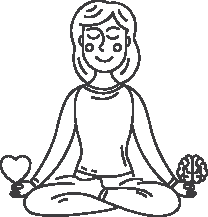
\includegraphics[scale=1.5]{willpower/ch8/1.pdf}
\end{figure}

\textbf{Пачаць можна прасьцей.} Для атрыманьня карысьці ад мэдытацыі ня трэба купляць фігурку Буды ці адразу зьяжджаць на працяглую віпасану. У гэтым разьдзеле мы з~вамі разьбяромся ў~базавых паняцьцях усьвядомленасьці, даведаемся яе нэўрабіялягічныя мэханізмы, вывучым, як яна ўплывае на фізычнае і псыхічнае здароўе. Таксама разьбяром асноўныя кампанэнты ўсьвядомленасьці, асвоім практычныя навыкі фармальнай і нефармальнай практыкі~--- ад усьвядомленай хадзьбы да дыхальнай мэдытацыі. Мне хочацца, каб мае словы не стваралі ў~вас ілюзію разуменьня, а~былі адно кіраўніцтвам да дзеяньня. Бо ўсьвядомленасьць~--- гэта перадусім практыка, а~ня гутарка, таму зразумець яе можна, толькі выконваючы практыкаваньні і заданьні. Доўга апісваць яе~--- гэта як чытаць пра сэкс або танцы: адно множыць памылкі. 

\emph{Як добра заўважыў адзін з~практыкаў пра ўсьвядомленасьць: ``Вельмі рэкамэндую практыкаваць, але не магу сказаць, навошта''.}

\subsection*{Ачышчэньне сьвядомасьці}

Бывае так, што ў~чалавека ў~галаве такія кепскія, цяжкія, брудныя і трывожныя думкі, што ён ня можа заставацца сам-насам з~сабою. Тады ён зьбягае з~рэальнасьці з~дапамогай наркотыкаў усіх відаў, ад хімічных допінгаў да занурэньня ў~фантазіі і фанатычнага захапленьня ідэямі. Многія кажуць, маўляў, я хачу ``пашырыць сьвядомасьць'', але гэта небясьпечна разбурэньнямі, бо сьцены гэтыя~--- апорныя. Сьвядомасьць, як месца знаходжаньня нашага Я, трэба не пакідаць ці пашыраць, а~чысьціць.

Многія людзі так баяцца застацца сам-насам са сваімі думкамі, ажно аддаюць перавагу ў~дасьледаваньнях удару электрычным токам, абы не адмаўляцца ад тэлефона. Пастаянная занятасьць таксама можа быць толькі ўцёкамі ад рэальнасьці. Хочаце ацаніць рэальную якасьць свайго жыцьця? Проста пасядзіце, нічога ня робячы, сам-насам са сваімі думкамі. Унутраныя адчуваньні й пакажуць ваш стан.

\textbf{Калі вам трапіла пляма бруду на адзеньне, вы не пачынаеце размазваць яго, піць з~гора або выкідваць адзеньне? Вы проста адціраеце пляму.} Даглядайце сьвядомасьць так, як вы мыеце валасы і чысьціце зубы. Эмацыйная гігіена і ўвага да сваіх думак~--- гэта важная частка здароўя і аснова гарманічнага стану. Няхай ваш розум будзе прыемным домам, дзе хочацца жыць, дзе добра знаходзіцца ў~цьвярозым і ясным стане, дзе вы можаце быць сумленным самі з~сабой і заставацца сам-насам з~самымі глыбокімі сваімі думкамі, а~ня бегчы ад іх.

\subsection*{Павышэньне ўзроўню ўсьвядомленасьці}

Калі вам цяжка апісаць свае эмоцыі, вы ўвесь час адцягваецеся, спрабуеце здушыць свае думкі, не заўважаеце свайго цела і адчуваньняў, адзначаеце складанасьці з~канцэнтрацыяй, схільныя імпульсіўна рэагаваць на свае пачуцьці ці ўчынкі іншых людзей, часта ловіце сябе на дзеях і ўчынках на «аўтапілёце», забараняеце сабе думаць пра «няправільныя» рэчы, вам цяжка заўважаць адценьні ў~прыродзе і дэталі на працы, вы ўвесь час спрабуеце выправіць мінулае ці фантазіруеце аб будучыні, то ў~вас, імаверна, нізкі ўзровень усьвядомленасьці, і гэты разьдзел дапаможа вам яе падняць. Упэўнены, што ўсьвядомленасьць~--- гэта адзін з~самых важных ``мяккіх навыкаў'' для кожнага чалавека.

\infobox{Усьвядомленасьць робіць наш розум гнуткім, а~гнуткасьць карысная для здароўя, няхай гэта будзе мэтабалічная~--- лёгкае пераключэньне паміж тлушчамі і вугляводамі, фізычная~--- добрая расьцяжка, або кагнітыўная~--- гаворка пра адаптыўнасьць.}

Для захаваньня псыхічнага здароўя важна ўмець хутка і лёгка пераключацца з~адной думкі на іншую, своечасова мяняць свае паводзіны. Пры хранічным стрэсе ўсьвядомленасьць зьмяншаецца і людзі становяцца кагнітыўна «цьвёрдымі». Няўменьне своечасова адпачыць, паклапаціцца пра сябе, распазнаць праблему~--- усё гэта прыводзіць да выгараньня і трывожнасьці. Людзей мардуе ня столькі сам стрэс, колькі іх кагнітыўная жорсткасьць. Практыка ўсьвядомленасьці павялічвае і вашу гнуткасьць, і адаптыўнасьць да зьменаў.

\emph{У працэсе эвалюцыі мы адаптаваліся да пастаянных пераменаў дзейнасьці: цыркадныя рытмы, цыклі актыўнасьці, харчовыя вокны і шматлікае іншае. Таму так важна правільна балянсаваць паміж працаваць/адпачываць, рухацца/сядзець, есьці/пасьціцца, зарабляць/траціць, браць/аддаваць, ствараць/спажываць, быць рэактыўным/быць праактыўным, быць аднаму/сярод людзей, рабіць кароткатэрміновае/рабіць доўгатэрміновае, транжырыць/інвэставаць, крытыкаваць/падбадзёрваць, клапаціцца пра сябе/клапаціцца пра іншых.}

\begin{figure}[htb!]
  \centering
  
\includegraphics[scale=1.5]{willpower/ch8/2.pdf}
\end{figure}

Практыка ўсьвядомленасьці дапаможа вам нашмат больш эфэктыўна спраўляцца з~нарастальнай нагрузкай, захоўваць сваю ўвагу і фокус на важных для вас рэчах і пры гэтым не забываць пра патрэбы свайго цела. Чым лепш вы трымаеце балянс, тым больш упэўнена пачуваецеся ў~новым сьвеце нарастальнай нявызначанасьці. Цікаўнасьць да сябе і цікавасьць, павага да свайго цела, думак, добрае і міласэрнае стаўленьне да сябе~--- гэта добры пачатак для практыкі ўсьвядомленасьці. Даведайцеся пра сябе лепей, надайце сабе ўвагу і стаўцеся да сябе болей сьвядома.

\subsection*{Пытаньні і заданьні}

1. Як часта і куды вы спрабуеце ``ўцячы'' ад непрыемных думак?

2. Ці добра вы разумееце эмоцыі, якія адчуваеце?

3. Заўважайце моманты, калі вы дзейнічаеце на аўтапілёце.


\section{Што такое ўсьвядомленасьць і як яе ўмацаваць?}

Многія людзі ўспрымаюць усьвядомленасьць і мэдытацыі як нейкую веру ці рэлігію, але гэта ня так. Усьвядомленасьць~--- гэта ў~першую чаргу трэніроўка мозгу: практыкуючыся, мы прапампоўваем сувязі паміж нэўронамі, умацоўваем нашу ўвагу гэтак жа, як нарошчваем мускулатуру ў~спартовай залі.

\textbf{Усьвядомленасьць~--- гэта форма самарэгуляцыі, здольнасьць канцэнтраваць безацэначную ўвагу на сваіх фізычных і разумовых працэсах.} У яе ёсьць і іншыя назвы: прыняцьце, увага, уважлівасьць, майндфулнэс.

\textbf{Усьвядомленасьць}~--- гэта бесьперапыннае адсочваньне бягучых перажываньняў, стан, у~якім вы факусуецеся на пражываньні толькі цяперашняга моманту, імкнучыся не адцягвацца на падзеі мінулага або думкі пра будучыню, знаходзячыся ``тут і цяпер''. Калі мы практыкуем усьвядомленасьць, то вучымся наўмысна накіроўваць сваю ўвагу на розныя аспэкты існага моманту. Наўмысна~--- гэта значыць, што мы прыкладаем намаганьне і засяроджваньне, каб пастаянна прысутнічаць у~сваім існым досьведзе, быць адкрытымі, успрымальнымі і адчуваць істую цікавасьць да сваёй сапраўднасьці-сучаснасьці.

\infobox{У выніку гэтай практыкі зь цягам часу мы вучымся ўспрымаць рэальнасьць бяз фільтраў розуму, бачыць сьвет такім, які ён ёсьць цяпер.}

Як вы робіце практыкаваньне з~гантэлямі? Факусуецеся на тэхніцы, падымаеце і апускаеце вагу пэўную колькасьць разоў. Дакладна гэтак жа і з~усьвядомленасьцю, толькі замест узьняцьця-апусканьня цяжару вы ловіце-вяртаеце ўвагу. Практыкуючыся, вы кожным разам нагадваеце сабе, што цяпер робіце і для чаго, трэніруеце пільнасьць: заўважаеце, калі адцягнуліся, і вяртаеце ўвагу да аб'екта засяроджваньня~--- дыханьне, цела, думкі і да т.~п.

\subsection*{Кампанэнты ўсьвядомленасьці}

Для прагрэсу ў~спартовай залі неабходны шэраг навыкаў: трэба вывучыць тэхніку практыкаваньняў, скласьці плян трэніровак, карэктаваць харчаваньне. Калі мы разьвіваем усьвядомленасьць, то зьвяртаем асаблівую ўвагу на \textbf{наступныя чатыры навыкі}: 
\begin{itemize}
  \item \textbf{навык назіраньня}: наколькі добра і ўважліва вы можаце заўважаць зьмены ўнутры сябе і звонку;
  \item \textbf{навык апісаньня досьведу}: уменьне дзеяць з~усьвядомленасьцю;
  \item \textbf{безацэначнае стаўленьне да свайго ўнутранага досьведу}: калі мы не чапляем ярлыкі і катэгорыі, а~прымаем зьявы такімі, якія яны ёсьць;
  \item \textbf{навык безрэакцыйнага стаўленьня}: калі мы ўстрымліваемся ад аўтаматычнага ўмяшаньня ў~назіраны намі працэс.
\end{itemize}

Калі вам нахамілі, вы зможаце заўважыць, як словы запускаюць у~вашым розуме і целе зваротную рэакцыю, і ўстрымацца ад аўтаматычнай рэакцыі, ператварыўшы звыклыя самашкадаваньне ці агрэсію ў~трансфармавальныя спакой і любоўнае спачуваньне.

\infobox{Не навешваючы цэтлікі на іншага чалавека, мы пакідаем яму і сабе магчымасьць зьмяніцца і паступіць інакш.}

\subsection*{Факусоўка ўвагі}

\textbf{Навошта факусаваць увагу?} Калі трэніроўкі ўмацоўваюць цягліцы і павялічваюць трывушчасьць, то практыка ўсьвядомленасьці павялічвае памеры шэрагу структураў мозгу, павялічвае іх актыўнасьць, дапамагае выразьней факусаваць прамень увагі.

\textbf{Уменьне накіроўваць сваю ўвагу можа радыкальна павысіць пасьпяховасьць вашых дзеяў.} Навык кіраваньня ўвагай значна ўплывае на прадуктыўнасьць, бо ён можа быць ужыты да любой задачы~--- ад уменьня даваць рады стрэсу і пераяданьню да міжасобасных адносінаў і прафэсійных задач.

Уявіце сабе навык увагі ў~выглядзе павелічальнага шкла. Сонечныя прамяні падаюць раўнамерна на ўсе прадметы~--- так і нашая ўвага расьсейваецца, ня надта ўплываючы на навакольны сьвет. Але лінза можа сабраць прамяні ў~адным пункце, што прывядзе да нагрэву і зьяўленьню полымя. Так і нашая ўвага, сабраная з~дапамогай прэфрантальнай кары ў~адным пункце, прывядзе да посьпеху ў~нашай працы і прагрэсу ў~самаразьвіцьці.

\begin{figure}[htb!]
  \centering
  
\includegraphics[scale=1.5]{willpower/ch8/3.pdf}
\end{figure}

\subsection*{Нэўрабіялёгія ўсьвядомленасьці}

Для больш эфэктыўнай прапампоўкі цягліцаў карысна ведаць іх анатомію. Усьвядомленасьць узьнікае ў~пэўных структурах мозгу. Розныя аддзелы мозгу аб'ядноўваюцца ў~функцыянальныя нэўронныя сеткі або контуры. Зьмена рэжыму мысьленьня зьвязана са зьменай актыўнасьці гэтых нэўронных сетак.

Калі вы занятыя працай, актыўная \textbf{цэнтральная выканаўчая сетка}, якая адказвае за кантроль рэакцыі на розныя стымулы, рашэньне пэўных задач у~паўсядзённым жыцьці.

Калі вы ўважліва чытаеце гэтую кнігу, то актыўная \textbf{саліентная сетка}, якая адказвае за ўсьвядомленасьць і ўвагу, аналіз сыгналаў, пазнавальныя і эмацыйныя функцыі, уменьне выбіраць з~плыні інфармацыі найважнейшае.

Калі вы проста ляжыце на канапе і нічым не занятыя, то актывуецца сетка пасыўнага рэжыму працы мозгу, яна ж нэўронная сетка апэратыўнага спакою ці \textbf{дэфолтная сетка}. Яна можа ўключацца і пры выкананьні аўтаматычных дзеяньняў, якія не патрабуюць увагі. Напрыклад, калі вы едзеце за стырном і круціце на аўтамаце розныя думкі ў~галаве.

\textbf{Сетка пасыўнага рэжыму працы мозгу} актыўная ў~плода пачынаючы з~30 тыдня. Яна ўключаецца, калі вы бязьдзейнічаеце, занураныя ў~думкі, мроіце наяве, факусуючыся на перажываньнях адносна вашай асобы. Можна сказаць, што гэтая сетка зьяўляецца цэнтрам «эга», яна прымярае ўспаміны і фантазіі да вашай асобы, фармуе аўтабіяграфію, самаацэнку, зьвязаная з~маральна-этычнымі ацэнкамі ды эмпатыяй. Яна можа дапамагчы ствараць, крэатывіць, прыдумляць незвычайныя рэчы. Мозг з~актыўнай сеткай пасыўнага рэжыму канструюе розныя сытуацыі будучыні і мінуўшчыны, робіць прагнозы. Марыць і фантазаваць карысна, але занадта высокая актыўнасьць сеткі спакою шкодная.

\textbf{Павышаная актыўнасьць сеткі спакою} павялічвае зацыкленасьць на сабе. Мы адчуваем гэта як бязмэтнае блуканьне розуму, разумовую жуйку, яна ўключае пракручваньне думак-прусакоў, асьцярогі, страхі. Часам сетку спакою называюць «унутраным тэлевізарам», які трэба выключыць. Чым больш вы сфакусаваныя на ўнутраным дыялогу, тым горшая ваша эмацыйная ўспрымальнасьць і здольнасьць вырашаць рэальныя задачы. Чым больш мы думаем пра сябе, тым больш няшчасным робімся. У дасьледаваньнях паказана, што больш высокі ўзровень аўтаматызму і блуканьня розуму зьвязаны зь меншай задаволенасьцю і ўзроўнем шчасьця. У людзей з~дэпрэсіяй назіраецца падвышаная актыўнасьць сеткі спакою, і яны ня могуць яе выключыць, вырашаючы пэўныя задачы.

У будызьме гэтую зьяву параўноўваюць з~розумам, «напоўненым п'янымі малпамі, якія кідаюцца з~галін дрэваў, скачуць і балбочуць не сьціхаючы». У шматлікіх духоўных практыках і псыхалягічных падыходах часта кажуць пра «ўтаймаваньне эга», угамаваньне блуканьня розуму, прыпынку ўнутранага дыялогу. З навуковага пункту гледжаньня ўсё гэта абазначае практыку зьніжэньня залішняй актыўнасьці сеткі спакою.

\subsection*{Як утаймаваць розум?}

Нэўронныя сеткі ня могуць быць актыўныя адначасова, яны працуюць у~супрацьфазе. Калі мы знаходзімся ў~стане патоку, сканцэнтраваныя на важнай і цікавай працы, гэта задзейнічае і ўмацоўвае нашу цэнтральную выканаўчую сетку і зьніжае актыўнасьць сеткі спакою.

\textbf{Невыпадкова раней выкарыстоўвалі такі мэтад лячэньня, як працатэрапія.}

Калі мы практыкуем усьвядомленасьць, адсочваем нашы думкі і рэакцыі, гэта задзейнічае сетку выяўленьня значнасьці і зьмяншае актыўнасьць сеткі спакою. Гэтае зьніжэньне і пераключэньне на іншыя сеткі вядзе да «ўгамаваньня розуму» і дазваляе вам стаць больш сабранымі, сьвядомымі, больш уважлівымі ў~жыцьці і працы. Цікавая праца з~годнымі задачамі і практыка ўсьвядомленасьці~--- найлепшыя прылады для кіраваньня сваімі сеткамі.

\subsection*{Прапампаваны мозг}

Як фізычная трэніроўка ў~любым узросьце ідзе на карысьць цягліцам, так і мозг можа зьмяніцца дзякуючы эфэкту нэўраплястычнасьці. Практыкаваньні на трэніроўку ўсьвядомленасьці дабратворна ўплываюць на розныя аддзелы мозгу, а~таксама на таўшчыню кары вялікіх паўшар'яў. Адсочваць прагрэс можна па ўстойлівасьці ўвагі ў~кагнітыўных тэстах, а~таксама з~дапамогай адмысловых нэўрагарнітураў (Muse, Neuralink і інш.).

\emph{Будыйскія манахі, напрыклад, дэманструюць недасяжную для большасьці звычайных людзей асаблівую высокачастотную гама-актыўнасьць мозгу, якая ўплывае на глыбіню сьвядомасьці.}

\subsection*{Характарыстыкі ўвагі}

Мы можам ацаніць увагу па глыбіні канцэнтрацыі, па ўстойлівасьці, па яе разьмеркаваньні і пераключэньні. Увага працуе ў~розных рэжымах: \textbf{агульная ўвага}~--- калі мы заўважаем мноства розных дэталяў і іх аналізуем, \textbf{сфакусаваная ўвага}~--- гэта здольнасьць устойліва канцэнтравацца на асобных дэталях. Усьвядомленасьць трэніруе абодва рэжымы і паляпшае іх узаемадзеяньне. Таксама прапампоўваецца і навык мэта-ўважлівасьці, то бок мы вучымся заўважаць моманты, калі адцягваемся. Зрэшты, асьцерагайцеся занадта старанна ацэньваць сябе і сваю мэдытацыю, таму што тады губляецца сэнс усьвядомленасьці, мы перастаём успрымаць рэчы такімі, як яны ёсьць.

\subsection*{Як практыкаваць усьвядомленасьць?}

Першасна гэта рэлігійныя будысцкія практыкі, але ў~заходніх краінах цяпер пераважае сьвецкі падыход да практыкі ўвагі, як да своеасаблівай мэнтальнай трэніроўкі. Гэта нескладана, тут няма посьпеху ці няўдачы, галоўнае~--- настойлівасьць і цікавасьць. Як жартуюць трэнеры, у~мэдытацыі самае складанае~--- знайсьці на яе час. Ня бойцеся, што практыка ўсьвядомленасьці памяняе ваш характар радыкальна: вы ня зробіцеся супэраптымістам ці, наадварот, дэпрэсіўным~--- пры дэпрэсіі практыка ўсьвядомленасьці наогул проціпаказаная. Да ўсіх мэаўт ва ўсьвядомленасьці варта падыходзіць перадусім пазітыўна і са спагадай да сябе: «Я малайчына, зрабіў/зрабіла невялікі крок, заўтра паспрабую яшчэ».

Практыкаваць усьвядомленасьць можна як фармальна (штодзённыя мэдытацыі), так і нефармальна (калі вы гуляеце, ясьце, працуеце і да т.~п.). Два найважнейшыя аспэкты практыкі на першым этапе, на якія я раю зьвярнуць асаблівую ўвагу,~--- гэта \textbf{навык накіроўваць і ўтрымліваць увагу на цяперашнім моманце і безрэакцыйнае стаўленьне да свайго досьведу.} Калі вы нязграбна пасьлізнуліся, утрымайцеся ў~моманце цяпер, а~ня думайце, як выглядаеце збоку, і ня лайце сябе за нязграбнасьць. Калі складана зрабіць гэта адразу, паспрабуйце для пачатку глядзець на непрыемныя сытуацыі постфактум, пытаючыся ў~сябе, дзе быў той момант, калі я на аўтамаце на кагосьці сарваўся?

\subsection*{Пытаньні і заданьні}

1. Ацаніце сваю здольнасьць факусаваць увагу. Вы можаце зрабіць гэта адвольна на любой тэме альбо толькі на важнай для вас? Колькі часу вы можаце падтрымліваць канцэнтрацыю на цікавым заданьні? А на нецікавым?

2. Сфакусуйцеся на працы. Складаныя цікавыя задачы карысныя для мозга. Успомніце сваю дзіцячую захопленасьць!

3. Паспрабуйце пераключаць сябе. Усьвядомце розьніцу, калі вы сфакусаваныя на сваіх асабістых праблемах і калі вы думаеце пра беды іншых людзей.


\section{Чым карысная ўсьвядомленасьць для розуму і цела}

Як пражыць у~тры разы даўжэй? Усьвядомленасьць~--- адзін зь нямногіх спосабаў гэта зрабіць. Бо калі мы праводзім гады на аўтапілёце, жывём у~сваіх думках у~мінулым ці будучыні, то рэальнае жыцьцё праходзіць нібы на паскоранай перамотцы. Жыцьцё на аўтапілёце пазбаўленае задавальненьня і не запамінаецца. Людзі на сьмяротным ложы часьцей за ўсё шкадуюць аб тым, што надавалі мала чыстай увагі зусім звычайным сытуацыям: сям'і, радасьці, адпачынку.

\infobox{Калі вы жывяце сьвядома дзьве гадзіны ў~дзень, то, павялічыўшы колькасьць усьвядомленых гадзінаў да шасьці, вы як быццам падоўжыце і сваё жыцьцё ў~тры разы.}

Усьвядомленасьць станоўча ўплывае ня толькі на псыхалягічнае здароўе, але й зьмяншае рызыкі шматлікіх захворваньняў. Імаверна, гэта адбываецца як праз эфэкт паніжэньня стрэсу, так і праз прыняцьце больш усьвядомленых і здаровых рашэньняў у~сваім жыцьці. Чым вышэйшая усьвядомленасьць, тым вышэйшая і прадуктыўнасьць чалавека~--- назіраецца дозазалежны эфэкт.

\emph{Параўнаньне розных праграмаў усьвядомленасьці паказвае, што для заўважнага станоўчага ўплыву на здароўе патрабуецца рэгулярная штодзённая мэдытацыя працягласьцю ня меней за 20--30 хвілінаў у~адзін ці два падыходы. Чым вышэйшая канцэнтрацыя ўвагі дасягаецца, тым вышэйшыя вынікі дае практыка.}

\subsection*{Здаровыя паводзіны}

Больш усьвядомленыя людзі менш схільныя да пераяданьня і курэньня, спажываньня алькаголю і наркотыкаў; праграмы ўсьвядомленасьці эфэктыўна дапамагаюць пазбавіцца ад залежнасьцяў. Усьвядомленасьць робіць вас больш аўтаномнымі і рацыянальнымі, а~працяглая мэдытацыя зьніжае аб'ём прылеглага ядра, і вы становіцеся больш незалежнымі ад узнагародаў. У адным з~дасьледаваньняў нават аднаразовая мэдытацыя ўплывала на прыняцьце больш аптымальных фінансавых рашэньняў і дапамагала ігнараваць прыроджаныя перадузятасьці і кагнітыўныя скажэньні.

\textbf{Увага}~--- гэта ня проста кагнітыўны навык, але й працэс зьмены мозгу. Калі нам нешта цікава, расьце ўзровень дафаміну, актывуюцца працэсы нэўраплястычнасьці, што вядзе да структурнай зьмены мозгу. Чым больш прыцэльную ўвагу вы можаце надаць сваім справам, тым хутчэй у~іх удасканальваецеся. А вось займаючыся гэтым жа, але безуважна, вы ніколі ня зможаце дасягнуць у~гэтай справе дасканаласьці.

\textbf{Практыка ўсьвядомленасьці паляпшае якасьць мысьленьня, дапамагае прапампаваць сацыяльныя, пазнавальныя і эмацыйныя навыкі.} Адбываецца ўзмацненьне кантролю прэфрантальнай кары над мігдалінай, таму мы лягчэй кантралюем эмацыйныя імпульсы, можам назіраць свае эмоцыі, а~ня быць паглынутыя імі, і самі вырашаць, паддавацца імпульсу ці не.

\emph{Як вы памятаеце, пры стрэсе часта адбываецца «крадзеж мозгу», але той, хто практыкуе ўсьвядомленасьць, рэдка страчвае кантроль над сабой.}

Чым лепш мы супрацьстаім імпульсам, тым гэта карысьней для нашых адносінаў і здароўя, тым больш слушныя рашэньні мы прымаем і тым лепш уяўляем сабе наступствы дзеяў. Таксама гэта вельмі важна, каб зьмяніць свае старыя звычкі. 

\emph{Памятаеце вядомы зэфірны тэст, які дасьледаваў тэму адтэрмінаванага задавальненьня? Здольнасьць дзяцей праяўляць цярплівасьць і супрацьстаяць спакусе вызначае іх посьпех у~далейшым жыцьці!}

\subsection*{Здаровае цела}

Практыка ўсьвядомленасьці аказвае магутнае ахоўнае ўзьдзеяньне на цела, павялічвае варыябельнасьць пульсу, тонус вагуса і ўзровень аксытацыну. Таксама яна зьвязаная і з~большым сардэчна-сасудзістым і мэтабалічным здароўем (вышэйшая адчувальнасьць да інсуліну, меншая рызыка дыябэту). Мэдытацыя зьніжае артэрыяльны ціск, паляпшае працу эндатэлію крывяносных сасудаў, памяншае раздражняльнасьць, трывогу і рызыку дэпрэсіі. 10-тыднёвая праграма мэдытацыі на 50\,\% паменшыла ўзровень успрыманага болю.

\emph{У дасьледаваньнях група паддосьледных, якія рэгулярна мэдытуюць, паказвае зьніжэньне сьмяротнасьці на 23\,\%, у~тым ліку і прыкметнае памяншэньне сьмяротнасьці ад пухлінавых і сардэчна-сасудзістых захворваньняў. Мэдытоўцы больш шчасьлівыя і задаволеныя сваім шлюбам, паводле дасьледаваньняў, у~іх на 11\,\% памяншаецца ўзровень стрэсу, зьніжаецца імавернасьць рэцыдыву дэпрэсіі.}

\begin{figure}[htb!]
  \centering
  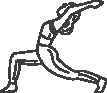
\includegraphics[scale=1.5]{willpower/ch8/4.pdf}
\end{figure}

Таксама мэдытацыя зьніжае ўзровень хранічнага запаленьня, вядзе й да прыгняценьня актыўнасьці запаленчага чыньніка NF-kB, дапамагае павысіць колькасьць CD4 + лімфацытаў у~ВІЧ-пацыентаў і павышае актыўнасьць тэламэразы. Уплыў мэдытацыяў на імунітэт дозазалежны, калі яны не былі штодзённымі і былі карацейшымі, чым 20 хвілінаў (у суме), то эфэкт быў слабы. \textbf{Пры вакцынацыі супраць грыпу ў~мэдытоўцаў выпрацоўваецца больш ахоўных антыцелаў у~параўнаньні з~тымі, хто не практыкуе. А чым больш антыцелаў~--- тым вышэйшы ўзровень імуннай абароны.}

\subsection*{Пабочныя эфэкты ўсьвядомленасьці}

Як і любы дзейсны мэтад, усьвядомленасьць мае свае пабочныя эфэкты. Так, яна можа пагоршыць стан пры шэрагу псыхічных разладаў, у~тым ліку некаторых відаў дэпрэсіі і біпалярнага разладу. Усьвядомленасьць~--- гэта ня спосаб рэляксацыі, а~дасьледзіны свайго розуму, таму часта яна можа павялічыць узровень трывогі. Пачынаць практыку трэба паступова, а~не з~працяглых рэтрытаў ці прасунутых тэхнік~--- такіх, як мэдытацыя на сьмерць, напрыклад. Пазьбягайце аўтарытарных «гуру» ўсьвядомленасьці і прасьвятленьня. Часта людзі выкарыстоўваюць практыку ўсьвядомленасьці для дасягненьня нейкага асаблівага ``прасьвятленьня''. Але такі падыход можа толькі прапампаваць нарцысізм.

\emph{Ёсьць жарт пра манаха, які прыгаворвае падчас мэдытацыі: «О, я так крута мэдытую! Я разбурыў сваё эга і ўціхамірыў свой розум! Хутка я стану самым прасунутым у~сваім храме!» Стаў лайк, калі пазбавіўся ацэначнага меркаваньня.}

У наш час нас усюды вучаць быць уважлівымі да сваіх эмоцыяў, да эмацыйнай усьвядомленасьці. Але залішняя заклапочанасьць сваім эмацыйным дабрабытам можа прывесьці да таго, што мы пачынаем пазьбягаць нэгатыўных эмоцыяў ці надаваць ім завялікае значэньне. Фіксуючыся на эмоцыях, мы пачынаем зьвяртацца да тых спосабаў рашэньня праблемаў, калі самаадчуваньне важнейшае, чым дасягненьне мэты. Гэта зьніжае нашу жыцьцеўстойлівасьць і робіць нас залішне адчувальнымі.

\textbf{Пераможцы думаюць пра дасягненьне мэты, нават нягледзячы на патэнцыйныя нэгатыўныя вынікі, а~астатнія думаюць аб тым, як камфортна сябе адчуваць. Таму так важна не прывязвацца да эмоцыяў і не ісьці на шворцы «добрых» адчуваньняў. Часам нашмат важней тое, што вы робіце, чым тое, што вы адчуваеце!}

Папулярнасьць усьвядомленасьці вядзе да таго, што яна часта скажаецца ці разумеецца няправільна. Напрыклад, людзі пачынаюць лічыць, што ўсьвядомленасьць мае на ўвазе пошук прычынаў усіх сваіх праблемаў унутры сябе і замірэньне з~навакольлем. Але гэта ня так. Наадварот, усьвядомленасьць дапамагае хутка разумець, калі прычынай пакуты зьяўляецца несправядлівасьць ці вонкавая агрэсія, і адэкватна рэагаваць на парушэньне межаў. Іншая памылковая думка, што ўсьвядомленасьць~--- гэта пра спакой розуму за кошт ігнараваньня або прыгнечаньня важных сыгналаў цела і псыхікі. Наадварот, яна дапамагае выявіць найважнейшыя свае адчуваньні й пачуцьці і дасьледаваць іх.

\textbf{Усьвядомленасьць~--- гэта ня ўцёкі ад рэальнасьці, а~набліжэньне да яе.} Усьвядомленасьць не зьвязаная з~культывацыяй абыякавага стаўленьня да сябе і іншых, яна неадзьдзельная ад дабрыні, любові і спагады. Усьвядомленасьць не зьвязаная з~ігнараваньнем доўгатэрміновых плянаў, адмаўленьнем самарэфлексіі і бестурботным жыцьцём у~стылі «жыві тут і цяпер, ня думай пра будучыню». Усьвядомленасьць~--- гэта ня спорт і не спаборніцтва ў~духу «хто круцей мэдытуе».

\subsection*{Пытаньні і заданьні}

1. Колькі гадзінаў на дзень вы губляеце на аўтаматычныя паводзіны?

2. Запішыце сваё жаданьне ці трывогу на аркушыку паперы і проста спакойна падыхайце, пабудзьце ў~цішыні ў~сапраўдным цяперашніммоманце. Вазьміце аркуш і прачытайце. Што зьмянілася?

3. Калі вы адчуваеце дыскамфорт, то памятайце, што ўсьвядомленасьць~--- гэта ўменьне ў~першую чаргу не ісьці на шворцы нэгатыўных думак і вытрымліваць іх. Усьвядомлена супраціўляйцеся нэгатыву і дыскамфорту, вырашаючы свае праблемы, і затым адпачывайце як чэмпіён.


\section{Хто крадзе нашу ўвагую і як стаць звышдрапежнікам}

Чаму тэма ўсьвядомленасьці робіцца такой папулярнай і запатрабаванай у~наш час? Навакольнае асяродзьдзе мяняецца, і за нашую ўвагу пачынае канкураваць усё большая колькасьць стымулаў, ад харчовых спакусаў да агрэсіўнай прапаганды. Калі мы не ўсьвядомленыя, то рэагуем на іх аўтаматычна і становімся падобныя на лялек-марыянэтак, якіх тузаюць за нітачкі. Разьвіцьцё ўсьвядомленасьці~--- гэта пытаньне выжываньня ў~сьвеце прывабаў і спакусаў, наш шлях да мэнтальнай свабоды.

Чаму ж мы схільныя марнаваць сваю ўвагу? Для нашага мозгу добра ўсё, што абяцае выжываньне і размнажэньне, але выжываньне ў~старажытныя часы залежала зусім ад іншых чыньнікаў, чым цяпер. Людзі сутыкаліся зь вялікай колькасьцю пагрозаў, таму важна было падтрымліваць згуртаваныя групы і хутка адказваць на агрэсію ці ратавацца ўцёкамі. А для нашага ўзнаўленьня вельмі важны сацыяльны статут, таму мы схільныя залішне рэагаваць на ўсё, што яму пагражае. Наш мозг зважае на ўсё, што абяцае стаць круцей, багацей, вядомей, а~таксама на ўсё, што можа прынесьці задавальненьне.

\subsection*{Лішак інфармацыі}

Сёньня за дзень чалавек можа атрымаць новай інфармацыі больш, чым раней за год. Апавяшчэньні ў~смартфонах, навіны ў~сацсетках, рэкляма на вуліцы~--- гэта крадзе нашую ўвагу, прычым усё больш агрэсіўнымі спосабамі. У ход ідзе дэманстрацыя грошай, эротыка, сэкс, улада, страх, сьмерць, фуд-порна~--- усё, што тузае за нашыя прыроджаныя нітачкі ўвагі да выжываньня і размнажэньня.

\textbf{Гэта вядзе літаральна да «эпідэміі безуважлівасьці», калі нашая ўвага распушчаецца сярод інфармацыйнага шуму.} Чым больш раздражняльнікаў на нас дзейнічае, тым цяжэй нам супрацьстаяць рэакцыі, і гэта спусташае нашу энэргію. Апошнім часам праблемы з~дэфіцытам увагі і гіпэрактыўнасьцю ўсё часьцей зьяўляюцца ня толькі ў~дзяцей, але і ў~дарослых. Так, за апошнія 10 гадоў колькасьць дарослых з~такімі праблемамі ўзрасла на 43\,\%. Дэфіцыт увагі выяўляецца як няўважлівасьць да дэталяў, складанасьць утрымліваць увагу падчас працы ці камунікацыі, няздольнасьць прытрымлівацца інструкцый, адцягвальнасьць, няпомнасьць, пазьбяганьне інтэлектуальна складанай працы.

\begin{figure}[htb!]
  \centering
  
\includegraphics[scale=1.5]{willpower/ch8/5.pdf}
\end{figure}

\textbf{Дык мо варта адмовіцца ад смартфонаў?} Вядома, тэлефоны ў~гэтым не вінаватыя. Калі мы ня ўмеем кіраваць сваёй увагай, то яе лёгка перахапляюць вонкавыя сыгналы, а~калі ўмеем, то самі выбіраем, куды ягенакіраваць. Калі мы не кіруем увагай, дык наш мозг~--- адно раб эмоцыяў, змушаны прыдумляць розныя гісторыі, каб растлумачыць сабе ж свае хаатычныя паводзіны і аўтаматычныя рэакцыі на вонкавыя стымулы.

\infobox{Усьвядомленасьць~--- гэта кіраваньне эмацыйным водгукам на вонкавыя стымулы, паўза паміж стымулам і рэакцыяй~--- вось дзе пачынаецца сапраўдная свабода.}

\subsection*{Як стаць звышдрапежнікам}

Гэта не пра расу Чужых, а~тэрмін зь біялёгіі, які пазначае жывёл на вяршыні харчовага ланцуга, якіх ніхто ня есьць, якія самі могуць адымаць чужую здабычу і нішчыць канкурэнтаў. Мне падабаецца мэтафара звышдрапежніка, бо яна досыць дакладна адлюстроўвае працэсы ў~дафамінавых аддзелах мозгу (перадусім у~стрыятуме), зьвязаныя з~працэсам «прысваеньня значнасьці». Розныя вонкавыя і ўнутраныя стымулы канкуруюць адно з~адным на адных і тых жа нэўронных контурах нашага мозгу. Які стымул перамагае, на той мы і рэагуем.

\textbf{Усе стымулы можна разьдзяліць на дзьве групы}: рэактыўныя (калі нешта вонкавае прыцягвае вашую ўвагу) і праактыўныя (калі вы самі вырашаеце, куды глядзець). Усьвядомленасьць трэніруе нашу праактыўную ўвагу і зьніжае рэактыўную.

Увага, як і сіла волі, рэсурс абмежаваны: для таго каб захаваць яе на праактыўнае ўмацаваньне, трэба перастаць марнатравіць і зьліваць яе на рэактыўнае рэагаваньне. Наша ўвага хоча ``зьесьці'' вялікую колькасьць ``драпежнікаў''. Драпежнік~--- гэта нейкі працэс, які спажывае нашую ўвагу і не дае наўзамен нічога карыснага. Напрыклад, бязмэтнае гартаньне стужкі, непатрэбныя імпульсіўныя пакупкі, прагляд коцікаў на ютубе. Калі вы заходзіце ў~фэйсбук для пошуку чагосьці канкрэтнага або для камунікацыі з~пэўным чалавекам (маючы фокус і мэту), то гэта будзе карысна.

\emph{Калі ж вы блукаеце бязмэтна, то непазьбежна станеце ахвярай алгарытмаў, якія падсоўваюць вам менавіта тое, што будзе зьядаць вашую ўвагу і высмоктваць энэргію. Вось вы паглядзелі навіны, эмацыйна спустошыліся, узбудзіліся і нічога важнага і карыснага для вас не адбылося.}

Калі хочаце прачытаць навіны ці праверыць пошту, задайце сабе праверачнае пытаньне: вы чытаеце навіны ці яны чытаюць вас? Пошта правярае вас ці вы правяраеце пошту? Адкуль ідзе імпульс?

Кіно, кнігі, інтэрнэт, палітыкі, прадаўцы тавараў і паслугаў канкуруюць і змагаюцца за каштоўны рэсурс~--- вашую ўвагу, прыдумляючы ўсё больш удасканаленыя спосабы яе захопу. Як і ў~выпадку наркотыкаў, заўсёды трэба павялічваць дозу, каб працавала. Падумайце, хто кіруе вашай увагай, што вас прыцягвае ці абіралі вы сьвядома рабіць тое, што вы робіце? А гэта важна, бо куды накіраваная ўвага, туды накіраваная і вашая энэргія.

\subsection*{Пытаньні і заданьні}

1. Якія стымулы мацней за ўсё чапляюць вас? Вы ведаеце чаму? Што дапаможа вам павысіць устойлівасьць да іх узьдзеяньня? Трэніруйце навык заўважаць, на што вы мацней за ўсё рэагуеце.

2. Прааналізуйце вашыя ўчынкі, дзе вы ўчыняеце рэактыўна, а~дзе праактыўна? Вы карыстаецеся смартфонам альбо ён карыстаецца вамі? Трэніруйце навык заўважаць, калі вы паддаяцеся вонкаваму ўплыву.

3. Што з~вашага навакольля мацней за ўсё крадзе вашую ўвагу? Што можна з~гэтым зрабіць? Трэніруйце навык прыбіраць са свайго асяродзьдзя тое, што замінае вашаму шляху да мэты, расчышчайце сабе дарогу і беражыце рэсурс увагі.


\section{Паўсядзённая ўсьвядомленасьць, або Як прачнуцца?}

«Прачніся, Нэа, ты ўграз у~Матрыцы»~--- такая фраза была зьвернутая да галоўнага героя вядомага фільма. Калі мы жывём на аўтапілёце, то нашае ўспрыманьне сьвету невыразнае, як быццам мы сьпім і ўсё адбываецца не па-сапраўднаму, ня з~намі. Практыкі ўсьвядомленасьці павялічваюць яснасьць і выразнасьць успрыманьня, мы як быццам абуджаемся ад сну і пачынаем бачыць рэчы і людзей такімі, якія яны ёсьць насамрэч.

\textbf{Чаму ж наш мозг не забясьпечвае нам такое ўспрыманьне па змоўчаньні?} Калі вы выставіце на смартфоне максімальную яркасьць, гучнасьць і відэадазвол, то батарэя хутка разрадзіцца і памяць перапоўніцца. Гэтак жа сама і з~мозгам. 

\textbf{Наш мозг~--- дзівосны орган зь велізарнай магутнасьцю: хоць ён займае 2\,\% масы цела, але можа паглынаць да 20\,\% усёй энэргіі.} Гэта шмат, таму падчас эвалюцыі выпрацаваліся рэжымы эканоміі пры апрацоўцы інфармацыі і прыняцьці рашэньняў. Ва ўмовах стрэсу няма часу старанна аналізаваць дэталі, трэба дзейнічаць як мага хутчэй, бо кожная сэкунда~--- гэта пытаньне жыцьця і сьмерці. Таму мозг аўтаматызуе мысьленьне і паводзіны. Аўтаматызацыя мысьленьня заключаецца ў~тым, што мы ацэньваем тое, што адбываецца, катэгорыямі, вешаем цэтлікі, ставім адзнакі без дэталёвага аналізу сытуацыі. Зразумела, калі навакольны сьвет пастаянны, гэта палягчае мысьленьне. 

\infobox{Цяпер сьвет так хутка мяняецца і становіцца такім складаным, што звычка ўсё ацэньваць на аўтамаце адно робіць мысьленьне неадаптыўным і звужае нашыя магчымасьці.}

Паступова такія адзнакі фіксуюцца ў~адзінай карціне сьвету, а~на ўзроўні мозгу~--- у~сыстэме сінаптычных сувязяў, якія адлюстроўваюць наш жыцьцёвы досьвед, а~не рэальны сьвет. Тое, што раней дапамагала выжыць, цяпер шкодзіць. Спрошчаная карціна сьвету, з~аднаго боку, аблягчае разуменьне, але й становіцца нашай турмой. Бо мы ацэньваем любую інфармацыю не бесстаронна, а~параўноўваючы яе з~фіксаванай ``карцінкай'' у~галаве і на аснове гэтага прымаючы рашэньні аб тым, што трэба рабіць. Атрымліваецца, мы дзейнічаем зыходзячы з~нашых уяўленьняў, а~не з~рэальных абставінаў.

\textbf{Перадузятасьць мысьленьня~--- гэта калі мы схільныя выбіраць толькі тое, што лепш упісваецца ў~нашу карціну сьвету, і ігнараваць астатняе.} Мозг можа выкарыстоўваць псыхалягічныя абароны, скажаючы ўспрыманьне. Напрыклад, мы абясцэньваем штосьці, што ў~нас не атрымалася. Пры стрэсе людзі могуць і зусім сыходзіць у~фантазіі. Але такая абарона адно шкодзіць, бо чым горшыя нашыя мадэлі сьвету і чым мацней яны адрозьніваюцца ад рэальнасьці, тым горш мы дзейнічаем і тым большы стрэс адчуваем. Такім чынам, аўтаматызм успрыманьня і дзеяньні прыводзіць да страты адэкватнасьці ўспрыманьня і выбару, у~выніку мы губляем магчымасьць разьвіцьця.

\textbf{У аўтаматычным рэжыме} мы дзейнічаем нягнутка, як робаты, можам выконваць пэўныя дзеяньні, нават не ўсьведамляючы іх. Такі аўтаматызм добры пры кіраваньні аўтамабілем або для боксу, але жыцьцё большае і разнастайнейшае, таму з~аўтаматызмам нам цяжка адаптавацца, мяняцца, пазбаўляцца ад звычак, якія адно замінаюць. Стрэсавыя рэакцыі, сьпешка, трывога, дэфіцыт рэсурсаў, жаданьне пазьбегнуць непажаданых эмоцыяў запускаюць і падсілкоўваюць аўтаматычнае рэагаваньне.

\begin{figure}[htb!]
  \centering
  
\includegraphics[scale=1.5]{willpower/ch8/6.pdf}
\end{figure}

Для нашага псыхічнага здароўя асабліва небясьпечнае аўтаматычнае рэагаваньне на думкі і эмоцыі. Тады нашыя рэакцыі ўтвараюць своеасаблівае ``пракрустава ложа'', пад якое мы падганяем навакольны сьвет, пастаянна знаходзячыся ў~параўнаньні ``жаданае-сапраўднае''~--- а~гэта часта выклікае фрустрацыю. Нават уласныя эмоцыі мы імкнёмся не прымаць, а~``вырашаць іх'', разьбірацца з~нэгатывам, напругай і стомаю. Але гэта толькі парадаксальным чынам узмацняе іх.

\infobox{Мы схільныя змагацца з~тым, што лічым няправільным, бо ``ў няправільным сьвеце нельга быць шчасьлівым''.}

\emph{У рэжыме дзеяньня мы прымаем рашэньні на аўтапілёце, імкнёмся ўсё прааналізаваць, змагаемся за зьмены, верым у~рэальнасьць нашых думак, пазьбягаем праблемаў і непрыемнасьцяў, думаем пра будучыню ці мінулае, нашыя рэсурсы спусташаюцца, мы прагнем утрымаць тое, што ў~нас ёсьць, адчуваем, што ўжо ўсё ведаем, і зьяўляемся экспэртам, шкадуем сябе, нудзімся ў~рутыне, ацэньваем усё навокал, раздражняемся, дзейнічаем фармальна, факусуемся на выніку, імкнёмся быць як усё. Пазнаяце сябе?}

У рэжыме ўсьвядомленасьці ўсё наадварот: мы робім усьвядомлены выбар, прымаем сьвет як ёсьць, ведаем, што нашыя думкі~--- толькі прадукт сьвядомасьці, набліжаемся да праблемаў і прымаем непрыемнае, жывём тут і цяпер, назапашваем рэсурсы, адпускаем непатрэбнае, глядзім на ўсё як першы раз, як пачатковец, добрыя да сябе, адчуваем цікавасьць, цярплівыя, даверлівыя, факусуемся на працэсе і дзейнічаем аўтаномна. Замест барацьбы з~рэальнасьцю мы прымаем яе без ацэнкі. Мы прызнаём, што рэчы і людзі такія, якія ёсьць, бяз спробаў іх зьмяніць. Мы прызнаём, што рэальнасьць і нашыя перажываньні могуць быць і непрыемнымі, і балючымі, што мы можам і прайграваць. Але назіраючы за гэтымі пачуцьцямі, мы можам эфэктыўна атрымліваць досьвед тут і цяпер, вывучаць іх, а~не асуджаць. Мы адмаўляемся ад прыгнечаньня ці сьвядомага кантролю эмоцыяў, але пры гэтым захоўваем магчымасьць не рэагаваць аўтаматычна на эмацыйныя імпульсы.

\subsection*{Зрабі паўзу}

Гэта самая простая практыка ўсьвядомленасьці~--- рабіць паўзы пасьля ўзьдзеяньня на вас якога-небудзь стымулу, пры гэтым можна ўдыхнуць-выдыхнуць і прыслухацца да сябе. Своечасова спыніцца~--- гэта амаль міні-мэдытацыя. Невялікая паўза паміж стымулам і рэакцыяй дапамагае нам усьвядоміць тое, што адбываецца, і зрабіць выбар.

\emph{Спытайце сябе перад прыняцьцем рашэньня: «Што мне трэба проста цяпер?», «Як канкрэтна я магу пра сябе паклапаціцца зараз?» і «Якое аптымальнае рашэньне з~улікам усіх абставінаў я магу прыняць?»}

\subsection*{Паўсядзённая ўсьвядомленасьць}

Паспрабуйце дадаць больш усьвядомленасьці ў~паўсядзённыя моманты жыцьця. Напрыклад, паўхвіліны ўсьвядомленасьці, калі вы спыніліся на сьвятлафоры. Я заўсёды ўспрымаю гэта як сыгнал запаволіцца, зважаю на сваё цела, эмоцыі, дыханьне. Практыкуйце ў~любы час, калі вам даводзіцца чакаць, асабліва калі нехта спазьняецца. Пачуцьцё раздражненьня~--- гэта паказьнік, што вы змагаецеся з~рэальнасьцю і знаходзіцеся ў~аўтаматычным рэжыме.

На працягу дня вяртайцеся да адчуваньняў цела. Якая ў~вас поза? Ці зручна вы седзіце? Як да вас дакранаецца крэсла, як стаяць вашы ногі на падлозе, ці камфортна вам? Памяняйце позу~--- гэта карысна ў~тым ліку для зьніжэньня нагрузкі на сьпіну. Рухайцеся ўверх па прыступках усьвядомленасьці: спачатку надайце ўвагу целу, затым эмоцыям, думкам, дзеям, мэтам, каштоўнасьцям.

\infobox{Выкарыстоўвайце вонкавыя напамінкі: усталюйце на тэлефоне (ёсьць адмысловыя праграмы), наляпіце стыкеры на экране~--- гэта будзе вяртаць вас ва ўсьвядомленасьць. Мяняйце напамінкі раз на тыдзень, інакш яны перастануць працаваць.}

\textbf{Дыханьне.} Як вы цяпер дыхаеце? Вяртайце ўвагу да свайго дыханьня часьцей~--- акрамя павелічэньня ўсьвядомленасьці, гэта яшчэ і магутная антыстрэсавага практыка. Вылучыце сабе прастору для ўсьвядомленасьці, напрыклад гаўбец, дзе вас нішто і ніхто не адцягвае.

\textbf{Усьвядомленая хадзьба.} Адчувайце, як рухаюцца і спружыняць вашы ногі, накіруйце фокус увагі ад ступняў да каленяў ці да дыханьня. Цалкам перанясіцеся ў~сапраўдны, цяперашні момант: адчуеце на скуры вецер і сонца, тэмпэратуру цела і паветра, будзьце ўважлівыя да таго, што вас атачае.

\begin{figure}[htb!]
  \centering
  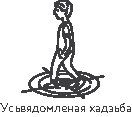
\includegraphics[scale=1.5]{willpower/ch8/8.pdf}
\end{figure}

\textbf{Усьвядомленае харчаваньне.} Зрабіце прыём ежы мэдытацыяй, адкладзіце тэлефон і не адцягвайцеся. Зьвярніце ўвагу на сваю ежу, як быццам вы бачыце яе першы раз: на пах, кансістэнцыю, вонкавы выгляд. Сфакусуйцеся на адчуваньнях і смаку, як яны мяняюцца ў~працэсе жаваньня, у~сярэдзіне і ў~канцы. Адчуйце, як рухаецца ваш язык, зубы. Адчуйце жаданьне праглынуць ежу, што суправаджае гэты працэс? Якія адчуваньні ў~жываце пасьля праглынаньня?

\begin{figure}[htb!]
  \centering
  
\includegraphics[scale=1.5]{willpower/ch8/7.pdf}
\end{figure}

\textbf{Зрабіце ўсьвядомлена неўсьвядомленыя дзеяньні.} Паспрабуйце сьвядома завязаць матузкі, пачысьціць зубы, папазіраваць перад люстэркам. Дадайце цікавасьці ў~«нясмачныя» пэрыяды вашага жыцьця. Часьцей пытайцеся ў~сябе, ці тое вы робіце, на што сыходзіць ваш час, ці сапраўды гэта вам трэба, ці можна зараз адрэагаваць інакш?

\textbf{Мыцьцё посуду або ўмываньне.} Паспрабуйце простыя хатнія справы рабіць так, быццам гэта нейкі сьвятарны рытуал. Напрыклад, мыйце посуд ня проста каб зрабіць яго чыстым, а~дзеля самога працэсу. Уявіце, што гэта не талеркі, а~каштоўныя сьвятыя статуі або прадметы мастацтва і што няма нічога больш важнага, чым зрабіць гэта. Падобным чынам можна зрабіць больш усьвядомленымі гатаваньне, умываньне ды іншыя справы.

\textbf{Усьвядомленае кіраваньне.} Як казаў Буда (але гэта не дакладна), «ты не затрымаўся ў~заторы, ты і ёсьць затор», або Сёе-тое пра любоўнае кіраваньне і стрэс у~заторы. Шкода затораў заключаецца ня толькі ў~павелічэньні часу сядзеньня, павышэньні ўзроўню выхлапных газаў (на 76\,\% вышэй, чым пры звычайнай язьдзе), самае шкоднае ўзьдзеяньне затораў~--- гэта стрэс і страта ўсьвядомленасьці. Узмацненьне стрэсу пры дарожных заторах нават атрымала асобную назву~--- traffic stress syndrome. Асабліва схільныя да небясьпекі асобы тыпу А. Стрэс у~заторы небясьпечны тым, што ён адносіцца да некантраляваных~--- то бок вы ня можаце пазбавіцца яго ці прадказаць працягласьць, ня можаце кантраляваць. Таму вельмі важна ў~гэтым выпадку браць нешта пад кантроль (дыханьне, цяглічную напругу) або практыкаваць зрушаныя паводзіны (слухаць музыку, навучальныя падкасты, весьці перамовы, стэлефаноўвацца зь сябрамі і да т.~п.).

Найлепшы варыянт, які я практыкую,~--- гэта сьвядомае кіраваньне. Практыка ўсьвядомленасьці мяркуе ўтрыманьне фокусу на сэнсарных перажываньнях: дыхальныя практыкі за стырном, факусаваць увагу на навакольным пейзажы. Але лепш за ўсё~--- любоўнае кіраваньне, калі мы замяняем імпульсы агрэсіі на іншых і сябе разуменьнем таго, што ўсе мы ў~гэтым заторы~--- людзі, усе мы пакутуем і ўсе мы хочам пазбавіцца ад пакуты. Пажадайце іншым пазбавіцца ад пакуты і быць шчасьлівымі, саступіце паласу. Усьміхніцеся суседу па паласе. У ісьце вы факусуецеся на ўсьведамленьні пакутаў і цяжкасьцяў іншых людзей, што дазваляе вам натуральным чынам стаць спагадлівымі, а~не крытычнымі як у~стаўленьні да іншых, так і ў~стаўленьні да сябе. Такая практыка павышае ўзровень станоўчых эмоцыяў, зьмяншае трывогу і стрэс.

\textbf{Усьвядомлены смартфон.} Дасьледаваньні паказваюць, што апавяшчэньні ад тэлефона ініцыююць узаемадзеяньне з~імі толькі ў~11\,\% выпадкаў, а~ў 89\,\% мы бяром яго самі. Многія людзі адзначаюць, што выкарыстоўваюць іх неўсьвядомлена, ня памятаюць, як бралі тэлефон у~рукі. Мы часта робім гэта неўсьвядомлена, рэфлекторна, пад узьдзеяньнем унутраных трыгераў. Зьвярніце сьвядома ўвагу, навошта вы бераце тэлефон. Магчыма, гэта ад нуды ці калі вы пачуваецеся няёмка. Мо тэлефон~--- гэта абарона або пазьбяганьне сваіх пачуцьцяў, пазьбяганьне камунікацыі? Спытайце сябе сумленна і ўсьвядомлена, навошта вы цяпер трымаеце тэлефон?

\textbf{Усьвядомленае чытаньне.} Калі вы чытаеце гэтыя радкі, зьвярніце ўвагу на шрыфт, фактуру паперы, прамежкі між словамі, пах паперы. Сфакусуйцеся на ідэях, зрабіце пазнакі на палях, канспэктуйце. У працэсе чытаньня праверце сябе: адкладзіце кнігу і паспрабуйце ўзнавіць апошнюю ідэю. Бо часта ўзьнікае ілюзія разуменьня, якая зьнікае, калі закрыць кнігу. Зрабіце гэта проста зараз! Чытаючы, зьвярніце ўвагу на сваю позу, на ўзьніклыя эмоцыі і адчуваньні.

\subsection*{Пытаньні і заданьні}

1. У якіх сытуацыях аўтаматызм лепш, а~разважаньні прытармажваюць вас? А ў~якіх наадварот? Як часта вы спрабуеце ``вырашыць праблему'' сваіх эмоцыяў, выправіць іх, замест таго каб проста дазволіць ім быць з~вамі?

2. Паспрабуйце заўважыць, як праяўляецца рэжым дзеяньня, напрыклад, у~ацэнках: як часта вы ацэньваеце людзей замест таго, каб заўважаць дэталі іх дзеяньня і паводзін? Усьвядомленасьць~--- гэта вызначэньне аб'ектыўных прыкметаў, а~не раздача суб'ектыўных ацэнак. Трэніруйце навык безрэакцыйнага ўспрыманьня.

3. У якіх паўсядзённых сытуацыях вам лягчэй за ўсё ўдаецца практыкаваць усьвядомленасьць? Вылучыце сабе ваш асабісты сьвядомы дзень або пару гадзінаў на бытавую ўсьвядомленасьць, каб практыкаваць усё, пра што гаварылася ў~гэтым разьдзеле. Трэніруйце навык зьвяртаць увагу на сваё цела, эмоцыі, думкі.


\section{Эмоцыі і ўсьвядомленасьць}

Да эмоцыяў шмат хто ставіцца з~пэўнай асьцярогай, прыгнятаючы і пазьбягаючы нэгатыву і баючыся некантраляванага запалу. Сапраўды, працяглыя нэгатыўныя эмоцыі ўплываюць на здароўе, як трапна заўважана, ``іржа есьць жалеза, а~смутак~--- сэрца''. У грамадстве прынята стрымліваць свае эмоцыі і ``валодаць сабой'', а~публічны паказ эмоцыяў часта лічыцца непажаданым. Эмацыйная ўсьвядомленасьць дапамагае нам знайсьці кампраміс: з~аднаго боку, прымаць любыя эмоцыі, ідэнтыфікаваць іх і бачыць прычыны, а~з другога~--- не рэагаваць на іх, не дазваляць эмоцыям зьліцца з~намі цалкам. Так мы захоўваем адчувальнасьць і кантроль адначасова.

У рэжыме дзеяньня мы часта спрабуем ``перамагчы'' эмоцыі, заглушыць іх. Такое выцісканьне ў~доўгатэрміновай пэрспэктыве можа прывесьці да нездаровых наступстваў, калі мы страчваем магчымасьць правільна распазнаваць, што ж мы насамрэч адчуваем. Узьнікае алексітымія~--- калі мы ня можам распазнаць, вытлумачыць або вэрбалізаваць адчуваньні, праява і перажываньне пачуцьцяў таксама выклікаюць цяжкасьці.

\textbf{Алексітымія} выяўляецца ў~няўменьні адрозьніваць эмоцыі і цялесныя адчуваньні, таму часта ў~алексітымікаў эмоцыі выяўляюцца ў~выглядзе боляў: ``Ты мне ціск падняў'', ``Мне ад цябе галава баліць''. Эмоцыі~--- гэта каталізатар для дзеяньня, менавіта дзякуючы эмоцыям мы праяўляем актыўнасьць, клапоцячыся як пра іншых, так і пра сябе. Алексітымікі маюць нізкі ўзровень самаўсьведамленьня і эмацыйнага інтэлекту, таму дрэнна разумеюць паводзіны і свае, і іншых людзей, у~выніку разьвіваецца сацыяльная дэзадаптацыя.

\begin{figure}[htb!]
  \centering
  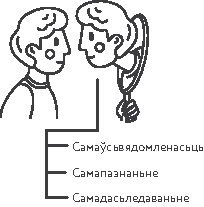
\includegraphics[scale=1.5]{willpower/ch8/9.pdf}
\end{figure}

\textbf{Ад 5 да 23\,\% здаровага насельніцтва маюць рысы алексітыміі, а~менавіта: праявы прыгнечаных эмоцыяў у~выглядзе боляў.}

\emph{Няўменьне выказваць і апісваць свае эмоцыі вядзе да множных цяжкасьцяў і парушэньняў. Алексітымія зьвязаная з~падвышанай рызыкай шызафрэніі, аўтызму, памежных разладаў асобы, псыхасаматычных захворваньняў, ужываньня наркотыкаў, парушэньняў харчовых паводзінаў, трывожных разладаў, гіпэртэнзіі, запаленчых захворваньняў кішачніка, мігрэні, паясьнічных боляў, астмы, фібраміалгіі і інш. Алексітымія ў~мужчынаў сярэдняга ўзросту (якім ``нельга плакаць'') зьвязаная з~двухразовым павелічэньнем сьмяротнасьці ад розных прычын, у~тым ліку няшчасныя выпадкі і злачыннасьць.}

Некаторыя аўтары лічаць, што алексітымія~--- гэта ахоўна-прыстасавальная рэакцыя ў~сучасных умовах, якая абараняе ад дэпрэсіі і выгараньня. Ацаніць узровень алексітыміі можна, прайшоўшы тэсты (таронцкая шкала і да т.~п.). Разьвівайце эмацыйны інтэлект, павялічвайце ўсьвядомленасьць і паважайце свае эмоцыі, выяўляйце эмоцыі спантанна і з~душой. Для пачатку можна пашырыць свой эмацыйны слоўнік~--- ці ўсе тыпы і адценьні эмоцыяў вы адрозьніваеце і ўмееце выказваць? Ну і, вядома, беражыце галаву~--- ня толькі ў~пераносным, але і ў~прамым сэнсе. Траўма галавы ў~шэсьць разоў павялічвае імавернасьць алексітыміі, як і хваробы Альцгаймэра, дарэчы.

\subsection*{Скіруйце ўвагу на вашыя эмоцыі}

Для паўсядзённай трэніроўкі эмацыйнай усьвядомленасьці зважайце на ўсе кампанэнты эмоцыі, выяўляйце іх і сытуацыі, у~якіх яны ўзьнікаюць. Прызнайце эмоцыі і не прыгнятайце іх, а~калі страшна, то прызнайце і гэта.

\textbf{Усьвядомце проста зараз:} 
\begin{itemize}
  \item Пра што вы думаеце, якія ў~вас \textbf{думкі}?
  \item Якія ў~вас \textbf{пачуцьці}?
  \item Які цяпер дамінуючы \textbf{імпульс}, што хочацца зрабіць?
  \item Якія цялесныя \textbf{адчуваньні}?
\end{itemize}

Разьвівайце навык уважлівасьці, кожны раз заўважаючы і называючы ўсе чатыры кампанэнты.

Зьвярніце ўвагу, як зьвязаныя паміж сабой цялесныя адчуваньні, імпульс, думкі, пачуцьці. У адказах пазьбягайце пасіўных апісаньняў, лепш казаць ня ``мне страшна'', а~``я адчуваю страх''. Для экспэрымэнту паназірайце, як зьменяцца кампанэнты эмоцыі, калі вы паўплываеце на адзін зь іх, напрыклад, выпрастаеце сьпіну, усьміхнецеся, прыдумаеце падбадзёрлівую мэтафару, сканцэнтруецеся на станоўчых пачуцьцях.

\infobox{Калі вы нічога не адчуваеце, не прыдумляйце тое, чаго не адчуваеце, магчыма, вам складана вызначыць эмоцыю ў~гэты момант, працягвайце назіраць.}

Цяпер, калі вы лепш усьведамляеце свае эмоцыі, нашмат лягчэй не паддавацца імпульсам. Прыдумайце зразумелую для вас мэтафару. Напрыклад, вашыя эмоцыі~--- гэта чаўны, на якіх сядзяць думкі, імпульсы, пачуцьці і цялесныя праявы, і яны праплываюць міма вас, а~вы седзіце на беразе. Вітайце як станоўчыя, так і адмоўныя эмоцыі. Ваш выбар~--- сядаць у~гэты човен ці не.

\emph{Магчыма, вам паасавацьмуць іншыя мэтафары: \textbf{кіно}~--- эмоцыі паказваюць на экране, а~вы~--- глядач у~зале, \textbf{аблокаў}~--- вы лежыце на зямлі, а~па небе праносяцца аблокі-эмоцыі, хваляў~--- вы з~дошкай для сэрфінгу стаіце на беразе мора і выбіраеце, якую хвалю прапусьціць, а~на якой эмацыйнай хвалі пракаціцца.}

\textbf{Здушэньне эмоцыяў.} Частую памылку робяць людзі, разьбіраючыся з~эмоцыямі. Калі мы задаём сабе пытаньне: ``Чаму мне так страшна?'' --- мозг можа знайсьці мноства тлумачэньняў. Аналізуючы кожную прычыну, мы яшчэ больш баімся і яшчэ мацней зацыкліваемся на гэтым. Калі вы спытаеце сябе: ``Чаму мне добра?'' --- таксама будуць знойдзеныя дзясяткі адказаў.

\emph{Паспрабуйце спытаць сябе, чаму ж вы такі лёсік, пашукайце прычыны. Зьвярніце ўвагу, як у~працэсе пошуку на вашым твары зьяўляецца ўсьмешка, выпростваюцца плечы, ясьнее ў~галаве. А цяпер зьверніцеся да сябе: чаму ж я такі няшчасны?~--- і пачніце над гэтым разважаць. Заўважылі розьніцу? Хоць рэальнасьць, у~якой вы знаходзіцеся, ані не зьмянілася.}

Душачы нэгатыўныя пачуцьці, мы душым сваю эмацыйную ўсьвядомленасьць цалкам. Уявіце сабе градку, дзе растуць і гародніна, і пустазельле. Немагчыма вырасьціць ураджай, каб побач не зьявіліся пустазельныя расьліны. Выполваючы пустазельле, мы закопваем іх побач з~гароднінай і яны служаць угнаеньнем. Так і нэгатыўныя эмоцыі ў~канчатковым выніку ідуць нам на карысьць, утвараючы тло, на якім больш прыкметнымі і прыемнымі становяцца радасьць і задавальненьне. Дык падзякуем ім за гэта.

\begin{figure}[htb!]
  \centering
  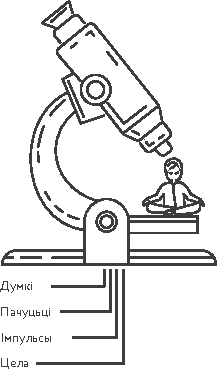
\includegraphics[scale=1.5]{willpower/ch8/10.pdf}
\end{figure}

Разьвіцьцё эмацыйнай усьвядомленасьці дапаможа вам павысіць ваш эмацыйны інтэлект. Заўважана, што менавіта ён у~многіх выпадках вызначае посьпех у~жыцьці. Толькі пачаўшы разумець і кіраваць сваімі эмоцыямі, вы зможаце разумець і ўзьдзейнічаць на эмоцыі і іншых людзей. У сучасным сьвеце EQ (эмацыйны інтэлект) становіцца больш каштоўным, чым IQ: на тле глабальнай рабатызацыі ўменьне распазнаваць чалавечыя эмоцыі~--- найважнейшы soft skill (гнуткі навык).

\subsection*{Пытаньні і заданьні}

1. Наколькі добра вы заўважаеце смагу, голад, сытасьць, напружаньне і іншыя праявы? Як яны праяўляюцца ў~целе?

2. Раздрукуйце сьпіс эмоцыяў. Паспрабуйце выказаць кожную, заўважаючы ўсе кампанэнты. Ці здольныя людзі ясна разумець вашыя эмоцыі? Згуляйце з~сябрамі ў~``пазнаваньне'' эмоцыяў адно аднаго.

3. Ці добра вы распазнаяце эмоцыі іншых людзей? Перад пачаткам гутаркі паспрабуйце вызначыць эмоцыі суразмоўцы і назваць іх.


\section{Розум пачаткоўца}

Калі працуеш над кнігай, старанна правяраеш кожную старонку. Але дастаткова іншаму чалавеку зірнуць, і ён зьлёту бачыць і памылкі друку, і іншыя памылкі, а~я дзіўлюся, як я сам гэтага не заўважаў. Наш погляд ``замыльваецца'', і мы страчваем сьвежасьць успрыманьня, калі шматкроць робім адно і тое ж. Розум пачаткоўца~--- гэта важны навык усьвядомленасьці, які дапамагае зірнуць на звыклыя рэчы сьвежым позіркам, пазбаўляючыся ад сваіх забабонаў і чаканьняў.

\emph{Мы ж праціраем брудныя пыльныя вокны, каб любавацца небам і дрэвамі, так і практыка ўсьвядомленасьці асьвяжае нашае ўспрыманьне рэальнасьці.}

Дзеючы аўтаматычна, мы даём усяму адназначныя ацэнкі і бачым адзіна слушны варыянт мысьленьня. Упэўненасьць у~гэтым вядзе да зьбядненьня нашага ўспрыманьня, замінае бачыць сапраўдную прыроду рэчаў і людзей, мы нібыта глядзім праз фільтр уласных ідэй, якім належыць быць людзям і зьявам.

Сярод лекараў ёсьць жарты пра вузкіх адмыслоўцаў, «сфэра ведаў якіх абмежаваная дыямэтрам трубкі, якую яны ўстаўляюць у~чалавека», і пра тое, што «вузкі спэцыяліст~--- гэта чалавек, які пазнае ўсё больш пра ўсё меншае і меншае, пакуль, нарэшце, не даведаецца ўсё ні пра што». Розум пачаткоўца валодае мноствам магчымых варыянтаў, ён гатовы вучыцца і мяняцца, а~розум экспэрта ўжо ўсё ведае і не гатовы мяняцца, а~толькі чапляецца за свае перакананьні.

\textbf{Розум пачаткоўца~--- гэта пра ўспрыманьне ўнікальнасьці кожнага моманту}, бо сапраўды~--- кожны момант нашага жыцьця новы, такога ніколі яшчэ не было, але ці здольныя мы заўважаць гэта? Гэта практыка ўсьвядомленасьці~--- глядзець на зьявы як быццам упершыню, успрымаючы іх цалкам і не адсякаючы нічога з~успрыманьня, выяўляючы неардынарнасьць звычайных рэчаў. Уявіце, што вы іншаплянэтнік, які ўпершыню на Зямлі і дзівіцца ўсяму, што ён бачыць. Куды вядзе вашая цікаўнасьць? Шукаць і ствараць новае можна заўсёды, нават адну і тую ж фразу можна сказаць з~рознымі адценьнямі, акцэнтамі ды інтанацыямі. Практыкуйце розум пачаткоўца ў~рутыннай працы~--- вашыя вынікі і задаволенасьць ад працэсу будуць павялічвацца. 

\infobox{Калі мы разумеем, што кожная сэкунда нашага жыцьця ўнікальная і больш ніколі не паўторыцца, то можам прасякнуцца ўдзячнасьцю да таго, як мы жывём і чаму цешымся.}

Прачынаючыся кожную раніцу, спытайце сябе, у~чым унікальнасьць менавіта гэтага дня і што вы можаце зрабіць, каб ён стаў яшчэ адным асаблівым днём вашага жыцьця.

\emph{Паспрабуйце ўключыць фантазію, каб дадаць навізны ў~звыклыя дзеі. Адзін з~настаўнікаў будызму прапануе ўявіць, што падчас прагулкі вы ідзяце не па дарозе, а~па пялёстках жывых кветак. Уявіце гэта сабе~--- і зьвярніце ўвагу, як зьмяніліся вашыя эмоцыі, думкі і хада.}

\begin{figure}[htb!]
  \centering
  
\includegraphics[scale=1.5]{willpower/ch8/11.pdf}
\end{figure}

\subsection*{Станьце дасьледнікам}

Падчас вучобы ў~мэдыцынскім унівэрсытэце ў~нас зь сябрамі была забаўка~--- седзячы на лаўцы, мы абмяркоўвалі мінака, прыкмячаючы ўсе мэдыцынскія дыягназы і асаблівасьці. Калі вы едзеце ў~грамадскім транспарце ці стаіце ў~заторы, патрэніруйцеся факусавацца на чым-небудзь на працягу некалькіх хвілінаў: адзначайце ўсе дробныя дэталі, паспаборнічайце зь сябрамі, хто зможа заўважыць больш.

\textbf{Калі мы гаворым пра ўсьвядомленасьць, то важнае менавіта само назіраньне, а~не высновы ці ацэнка.}

Мы трэніруем навык назіраньня: дасьледуйце ўсё, што адбываецца звонку і ўсярэдзіне вас, вашыя думкі і адчуваньні, дазвольце сабе ўсьвядоміць гэта. Уявіце, што вы навукоўца або дэтэктыў і проста зьбіраеце факты. Калі мы ўсьведамляем дэталі, то выносім у~сьвядомасьць шмат звычайна неўсьвядомленай інфармацыі, і ўжо гэта мяняе нашае да яе стаўленьне. Навучыцеся заўважаць, калі розум уключае кагнітыўныя фільтры і скажае рэальнасьць. Толькі ня стаўцеся да гэтага занадта сур'ёзна і захоўвайце пачуцьцё гумару й дасьледчай цікавасьці, не спрабуючы выправіць свае «няправільныя» рэакцыі.

\subsection*{Не сьпяшайцеся}

Наш мозг уладкаваны так, што ўсё новае і незразумелае павялічвае ўзровень дафаміну. А дафамін вызначае ня толькі цягу да навізны, але й жаданьне знайсьці прычынна-выніковыя сувязі, зьвязаць тканіну сьвету ў~адну карціну. Калі бярош кнігу пасьля блуканьняў па палях зь мікраскопам, яна здаецца адкрыцьцём, бо дае дакладныя адказы і тлумачыць усё, што ты бачыў, усё, што цябе зьдзіўляла. 

\emph{Мікраскоп мне прынёс тата, калі я вучыўся ў~пятым класе. Улетку мы жылі ў~вёсцы, і я проста выправіўся зь мікраскопам у~поле: у~кроплях вады я бачыў, як рачкі ядуць водарасьці, назіраў за раеньнем дафній, а~лязо дапамагала разгледзець дэталі будовы расьлінаў і казюрак. Перада мной як быццам раскрыўся цудоўны сьвет, яркі, незразумелы і прыцягальны. А вось урокі біялогіі ў~школе былі сьмяротна нуднымі.}

Спачатку табе расказваюць, што ты павінен убачыць, фармуючы чаканьне. Затым ты бачыш нашмат менш~--- рэальнасьць меншая за чаканьне, і дафамін ідзе ўніз. Ідэальна было б даваць магчымасьць разьвіваць цікаўнасьць, самім адчуць чараўніцтва адкрыцьцяў, напал цікаўнасьці, рызыку навізны і толькі потым, калі дзеці самі сфармуюць пытаньні адносна таго, што яны бачаць, адно тады растлумачыць і ўпарадкаваць. Атрымліваць веды трэба сьвядома, а~не як цяпер~--- калі іх сілком запіхваюць у~дзяцей, не пытаючыся іх згоды і не чакаючы гатовасьці. Тлумачачы занадта рана, мы забіваем навык задаваць пытаньні, забіваем жаданьне знаходзіць адказы і самае галоўнае~--- забіваем захапленьне навізной і цікаўнасьць.

\emph{Лінгвіст Ноам Хомскі ў~лекцыі «Адукацыя: каму і навошта» прыводзіць прыклад, як занадта раньні аповед пра ДНК забівае цікавасьць і жаданьне да гэтай тэмы ў~дзяцей у~той момант, калі яны не гатовыя яе зразумець: «Мы сапсавалі выдатную гісторыю, распавёўшы яе зарана».}

Было б выдатна, калі б, уваходзячы ў~новую сфэру, мы прыпыняліся, каб пасьпець зьдзівіцца, пазахапляцца, паламаць галаву, сфармуляваць пытаньні і захацець атрымаць на іх адказы. І толькі потым перайсьці непасрэдна да атрыманьня ведаў.

\subsection*{Пытаньні і заданьні}

1. Пачынайце і новы праект, і новы дзень з~чыстага аркуша. Не пераносьце цяжар клопатаў і трывог на свае новыя пачынаньні. Уявіце, што кожную раніцу вы нараджаецеся новым чалавекам, і ў~вас ёсьць магчымасьць зрабіць менавіта так, як вы хочаце.

2. Практыкуйце розум пачаткоўца ў~паўсядзённым жыцьці і ў~працы. Паглядзіце на праблему збоку, растлумачце яе іншаму чалавеку. Не хавайцеся за складанасьцю: як трапна заўважыў Фэйман: «Калі навукоўца ня можа растлумачыць васьмігадоваму хлопчыку, чым ён займаецца,~--- ён шарлатан».

3. Культывуйце цікаўнасьць. Спрабуйце новае, ідзіце, куды вас вабіць цікавасьць, купіце выпадковую кнігу, даведайцеся нешта, што выходзіць за межы вашае рутыны.


\section{Фармальная практыка. Дыхальная мэдытацыя}

Калі вы ўжо пачалі практыкаваць паўсядзённае ўсьвядомленасьць, то маглі заўважыць яе дабрадайнае ўзьдзеяньне. Але толькі рэгулярная паўсядзённая практыка мэдытацыі можа сапраўды глыбока і трансфармавальна паўзьдзейнічаць на вас. Мэдытацыя, як і лекі, працуе, калі прымаць яе кожны дзень увесь пэрыяд лячэньня. Добра практыкаваць усьвядомленасьць у~штодзённасьці, нефармальна, а~штодзённыя фармальныя практыкі патрэбныя, каб быў рост. 

\infobox{Як немагчыма напампавацца або схуднець за пару дзён, так ня варта чакаць прасьвятленьня праз 20 хвілін мэдытацыі. Але пастаянная яе практыка прынясе свой каштоўны плён.}

\subsection*{Сэанс мэдытацыі}

Вылучыце сабе ад 5 да 30 хвілін, знайдзіце спакойнае месца, дзе вы зможаце заставацца ў~расслабленай нерухомасьці. Адключыце тэлефон, папярэдзьце, каб вас не турбавалі, абярыце зручнае адзеньне. Поза для мэдытацыі можа быць любая, пры якой вы можаце захоўваць прамую сьпіну: сядзіце ўпэўнена, устойліва, з~захаваньнем увагі, годнасьці й пільнасьці. Рукі пажадана разгарнуць далонямі ўверх, сківіцы расслабленыя, вусны мякка самкнёныя, язык кранаецца нёба за верхнімі зубамі. Локці хай будуць распраўленыя, а~галава~--- роўна над хрыбтом. Сядзіце роўна, не адхіляючыся. Лепш не мэдытуйце лежачы~--- так вы можаце заснуць. Па першым часе няхай вашая мэдытацыя будзе кароткай, 5--10 хвілін. Ня варта мэдытаваць на працягу гадзіны-паўтары пасьля ежы і рабіць больш чым 1--2 сэсіі (з досьведам вашая практыка можа пашырыцца). Зважайце на зьмену свайго становішча і на станоўчыя адчуваньні, але не прывязвайцеся да іх і не рабіце сваёй мэтай. 

\textbf{Перад мэдытацыяй нагадвайце сабе, для чаго вы гэта робіце: ``Я мэдытую для ўмацаваньня ўвагі і буду сабраны і ўважлівы ў~мэдытацыі'' ці ``Няхай я буду шчасьлівы''.} Вельмі важна захоўваць энэргічнасьць, увагу, пільнасьць, не паддаючыся дрымотнасьці. Паназірайце за ваганьнямі фокусу ўвагі адносна гэтага моманту, не дазваляючы яму сасьлізгваць у~мінулае ці будучыню: вось ваша дыханьне, цела, думкі, гукі. Затым плыўна звужайце фокус толькі на сваім целе, выбраўшы дыханьне, цялесныя адчуваньні або думкі. Адчуйце посмак мэдытацыі, калі яе завершыце. Адзначце спакой і прымірэньне розуму і як затым яны зьмяншаюцца ў~звыклай плыні думак.

\emph{Часам мэдытацыя гострыць псыхалягічныя праблемы, бо шмат што пачынае выплываць на паверхню, і чалавек становіцца вельмі раздражняльным. У такім выпадку важна прымаць і такі вынік, гэта нармальна. Але калі мэдытацыя ўвесь час выклікае багата раздражненьня і ў~практыцы ўвесь час усплываюць нявырашаныя праблемы, то варта папрацаваць з~псыхолягам, каб спачатку расчысьціць сьвядомасьць.}

\begin{figure}[htb!]
  \centering
  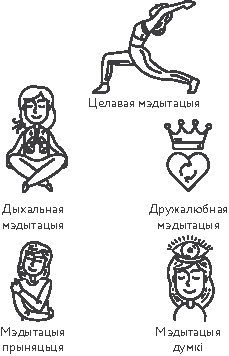
\includegraphics[scale=1.5]{willpower/ch8/12.pdf}
\end{figure}

\textbf{Дыхальная мэдытацыя}~--- гэта базавая тэхніка для практыкі ўсьвядомленасьці. Дыханьне ўнікальнае тым, што яно спантаннае і аўтаномнае, але мы можам браць яго пад кантроль. Дыханьне~--- гэта індыкатар ўзроўню стрэсу, перамыкач розных станаў. Сядзьце, сфакусуйце сваю ўвагу на дыханьні. Зрабіце пяць расслабляльных доўгіх удыхаў-выдыхаў, перастаньце кантраляваць дыханьне і пачніце за ім назіраць. У працэсе вы можаце факусаваць сваё дыханьне на розных частках, адзначайце адчуваньні пры ўдыху і выдыху ў~вобласьці ноздраў, грудзей, жываце, іншых частках цела. Звярніце ўвагу, як мяняюцца адчуваньні ў~целе на ўдыху і на выдыху, зьвярніце ўвагу на паўзы, якія разьдзяляюць ўдых і выдых.

Калі падчас мэдытацыі выплываюць непрыемныя думкі і эмоцыі, унутраныя камэнтары, то проста адзначайце, што адцягнуліся на іх, і вяртайце сваю ўвагу назад да дыханьня. Можаце пахваліць сябе, што хутка іх заўважылі, але ня варта лаяць сябе за гэта: адцягненьне і вяртаньне ўвагі~--- гэта неад'емныя часткі мэдытацыі. У канцы мэдытацыі хай увага ахопіць усё ваша цела адразу: уявіце, як вы ўдыхаеце і выдыхаеце ўсім целам адначасова. Утрыманьне ўвагі на дыханьні і зьяўляецца галоўнай мэтай мэдытацыі.

\subsection*{Пытаньні і заданьні}

1. Усталюйце дыхальную праграму на тэлефон, у~момант стрэсу проста дыхайце.

2. Выкарыстоўвайце нефармальную мэдытацыю, напрыклад кожны раз робячы некалькі павольных усьвядомленых дыхальных цыклаў, калі стаіце на сьвятлафоры, калі падымаецеся ў~ліфце, калі сядаеце за стырно або выходзьце з~машыны.

3. Зрабіце адзін сэанс дыхальнай мэдытацыі сёньня.


\section{Думкі і ўсьвядомленасьць}

Я люблю разглядаць аблокі, яны як нашыя думкі~--- неймавернай формы, рознага колеру і падобныя на мудрагелістыя вобразы. Я ведаю, што аблокі сыдуць пад узьдзеяньнем ветру, таму не спрабую іх разагнаць сам. Нават калі неба зацягнутае хмарамі, за імі заўсёды ёсьць яркае сонца і сіняе неба. Бывае, здаецца, што ў~жыцьці няма нічога, апрача цяжкіх і цёмных думак. Але гэта ня так~--- неба і сонца заўсёды чыстыя, і ўсьвядомленасьць дапамагае памятаць пра гэта ў~самыя цяжкія моманты.

\infobox{Згадайце гэты прыемны момант: калі ўзьлятаеш на самалёце ў~дождж ці сьнег, прайшоўшы праз аблокі, бачыш сонца і неба! Гэтыя сонца і неба ёсьць з~намі кожны дзень.}

Зьвярніце ўвагу на тое, як праходзіць працэс мысьленьня~--- мы ж пастаянна размаўляем самі з~сабой. Простае назіраньне паказвае, што нашыя думкі могуць нараджацца выпадкова і генэравацца мінулым досьведам, перажыванымі эмоцыямі, нашай ацэнкай сытуацыі, недасыпам і да т.~п. Асабліва заўважна гэта пры стрэсе або ў~стоме, калі зьяўляюцца тыповыя ``стрэсавыя'' думкі, якія звычайна зьнікаюць пасьля адпачынку.

\textbf{Гэта прыводзіць да важнага разуменьня: нашыя думкі ня тоесныя нам самім.} Мы не прымаем рашэньне адчуваць пэўны настрой або думаць нейкую думку~--- думкі нараджаюцца аўтаматычна, спантанна або пад вонкавым узьдзеяньнем. Думкі прыходзяць і сыходзяць, але вельмі часта пры нізкай усьвядомленасьці мы атаясамліваем сябе з~думкамі і рэагуем адпаведным чынам.

\textbf{Усьвядомленасьць вучыць заўважаць думкі} і ня быць захопленымі іх патокам, дапамагае зразумець, што ня мы генэруем нашыя думкі па жаданьні, што шлейфы думак~--- гэта адлюстраваньне і сума мноства нэўронных сетак. Мэтай такога ўнутранага дыялёгу зьяўляецца фармаваньне кансэнсусу ў~якім-небудзь пытаньні, мы можам пераконваць сябе нешта зрабіць ці не зрабіць, апраўдаць рашэньне, адказаць крыўдніку. Небясьпечна, калі мы ня можам гэтага зразумець, тады нават выпадковыя думкі могуць кіраваць нашымі рэакцыямі. Мозг часта стварае неадэкватныя мадэлі паводзінаў і ілюзіі, якія значаць для нас больш, чым рэальнасьць. Кагнітыўныя памылкі вядуць да павелічэньня стрэсу і пакутаў. А спробы зьмяніць мінулае ці паўплываць на няпэўную будучыню могуць толькі ўзмацняць стрэс.

\textbf{Павышэньне ўсьвядомленасьці паляпшае яснасьць мысьленьня, разбураючы ілюзіі.} Падчас практыкі ўсьвядомленасьці мы разьвіваем здольнасьць назіраць за сабой збоку, каб ня быць паглынутымі плыньню думак, вучымся ўсьведамляць свае парывы, лепей разумець эмоцыі.

\begin{figure}[htb!]
  \centering
  
\includegraphics[scale=1.5]{willpower/ch8/13.pdf}
\end{figure}

\emph{Мне падабаецца такая мэтафара. Уявіце сажалку з~чыстай вадой, у~якой відаць дно. Калі вы кінеце камень, то хвалі перашкодзяць бачыць дно. Каб ізноў атрымаыць празрыстасьць, трэба проста чакаць. А калі кідаць камяні ўвесь час, то можна вельмі моцна ўзбаламуціць ваду ў~сажалцы. Так і думкі віхруюць сумятню, парушаючы яснасьць розуму: чым больш думак мы пракручваем, тым мацней страчваем усьвядомленасьць.}

У норме \textbf{мэханізм унутранага дыялёгу}, размовы з~самім сабой~--- гэта карысны інструмэнт для самарэфлексіі, ацэнкі свайго досьведу і стану. Ён дапамагае рацыянальна ацэньваць сябе і свае дзеяньні, аналізаваць сытуацыю, разьбірацца ў~складаных паняцьцях у~рабоце і навуцы. А яшчэ~--- падтрымліваць сябе, падбадзёрваць, знаходзіць аргумэнты для дзеяньняў. Выяўляючы свае тыповыя думкі, зьвярніце ўвагу, ці дапамагаюць яны вам у~кожнай сытуацыі або толькі пагаршаюць яе.

\subsection*{Сумнявайцеся ў~каштоўнасьці думак}

Магчыма, гэта гучыць нязвыкла, але абсалютная большасьць нашых думак~--- проста шум: далёка ня ўсё, што ёсьць у~вашай галаве, гэта добрыя думкі. Маецца шмат такога, што замінае і шкодзіць, і гэтыя думкі трэба як шкоднікаў распазнаваць і прыбіраць~--- або аспрэчыць рацыянальна, або абсурдызаваць, высьмеяць.

\emph{Ідэальна, калі мы можам свайго ўнутранага крытыка замяніць на ўнутранага сябра, сябе-з-будучыні ці ўнутранага настаўніка, якія падтрымаюць нас і да якіх заўсёды можна зьвярнуцца па дапамогу.}

Калі наш унутраны дыялёг пачынае працаваць супраць нас, гэта можа выяўляцца ў~самых розных формах. Напрыклад, пры гіпэрактыўнасьці дэфолтнай сеткі спакою мозгу (блуканьне розуму) узьнікаюць аўтаматычныя нэгатыўныя думкі. Іх лёгка пазнаць: яны часта ўтрымліваюць абагульненьні (заўсёды, кожны, усё, ніхто, ніколі, усюды і да т.~п.), пачуцьцё віны (мусіш, павінная, абавязаны, трэба), акцэнтуюцца на нэгатыве (вы ня бачыце станоўчага ў~сытуацыі). Узьнікае поўная ўпэўненасьць у~разуменьні сытуацыі, аж да таго, што вы ``ведаеце'' думкі іншага чалавека. Важна разьвіваць безрэакцыйнае стаўленьне да такіх думак, каб не ісьці ў~іх на шворцы. Часам нашыя думкі здаюцца нам вялікімі, іх прыемна думаць і здаецца, што адно толькі думаньне~--- карыснае. Але такія настойлівыя думкі, што пастаянна выклікаюцца ва ўласнай галаве, і фантазіі могуць быць адным з~варыянтаў дафамінавай самастымуляцыі. 

\textbf{Калі вы ўвесь час ганяеце адныя й тыя ж думкі для задавальненьня, але яны не прыводзяць да рэальных зьменаў і вы зноў думаеце пра гэтыя ідэі для зьняцьця дыскамфорту, то гэта ня ёсьць здаровы спосаб мысьленьня. Спытайце сябе, навошта вы гэта робіце?}

\subsection*{Паспрабуйце паэкспэрымэнтаваць}

Напрыклад, набліжайцеся да таго, чаго вы імкнуліся пазьбягаць, адзначаючы зьмены сваёй плыні думак. Запісвайце думкі стасоўна якой-небудзь сытуацыі, затым спраўджвайце іх на рэальным становішчы рэчаў. Аддаляйцеся ад нефункцыянальных думак, станьце бесстароньнім назіральнікам. Зразумейце, што такія думкі аўтаматычныя, сфармаваныя ў~мінулым ці навязаныя вам, гэта ня вашае Я. Усьвядомце, што гэтыя думкі замінаюць вам адаптавацца да рэальнасьці, сумнявайцеся ў~іх, калі яны не адпавядаюць рэальнасьці. Нават адны і тыя ж фізыялягічныя адчуваньні можна перамаркіраваць так, што гэта цалкам зьменіць іх ацэнку.

\emph{Напрыклад, стрэсавыя адчуваньні я ўспрымаю як магчымасьць, а~не перашкоду, адказнасьць, а~не трывогу, цікаўнасьць, а~не насьцярожанасьць, натхненьне, а~не хваляваньне.}

\subsection*{Мэдытацыя «думкі»}

Пачніце мэдытацыю з~дыханьня. Пераключыцеся на думкі, назірайце ўзьнікненьне і зьнікненьне думак у~розуме. Як быццам гэта аблокі плывуць па небе. Паспрабуйце заўважыць моманты іх узьнікненьня і распушчэньня. Не спрабуйце пазбавіцца думак або ісьці за імі, ня трэба спрабаваць падумаць аб нечым адмыслова. Часам думкі будуць вас зацягваць~--- заўважайце гэта і вяртайцеся назад. Калі думкі выклікаюць яркія эмоцыі, проста назірайце, не рэагуючы. Калі цяжка супрацьстаяць плыні думак, вяртайцеся да дыханьня, вяртайцеся да ўсьвядомленасьці і зноў пераключайцеся на назіраньне за разумоваю плыньню.

\subsection*{Пытаньні і заданьні}

1. Як часта плыня думак захоплівае вас і вы ідэнтыфікуеце сябе зь ёй? Ці прыводзіла гэта да праблемаў?

2. Ці падбадзёрваеце вы сябе альбо крытыкуеце ва ўнутраным дыялёгу? Многім спартоўцам падтрымальны ўнутраны дыялёг («Ты справісься!») дапамагае перамагаць.

3. Паспрабуйце «адкруціць назад» ланцужок думак, успомніўшы, ад якой думкі вы перайшлі да папярэдняй, а~ад яе~--- да яшчэ больш раньняй. Такое практыкаваньне паказвае, што хада думак часта зьвязаная з~выпадковымі асацыяцыямі.


\section{Прыняцьце}

\emph{Аднойчы Буду плюнуў у~твар незнаёмец, Буда проста выцерся і спытаў, ці ёсьць у~таго што дадаць. На просьбы вучняў адпомсьціць заўважыў, што не абразіўся, бо не прыняў гэты ўчынак на свой рахунак.} 

Дзеючы аўтаматычна, мы можам прымаць на свой рахунак тое, што ня мае да нас ніякага дачыненьня. Нехта сьмяецца, і мы думаем, што гэта з~нас, чуем ад сваякоў пра хваробы і пачынаем шукаць іх у~сабе. Зь іншага боку, часта мы адмаўляем рэчы, якія адбываюцца з~намі, свае асаблівасьці, праявы сваіх блізкіх і пратэстуем супраць рэальнасьці. Усё гэта вядзе да разбуральных наступстваў.

\textbf{З намі могуць здарацца розныя рэчы, але прымаць ці не прымаць іх~--- гэта таксама пытаньне навыку ўсьвядомленасьці.}

\subsection*{Прыняць рэальнасьць}

Калі рэальнасьць не адпавядае нашай карціне сьвету, нашым чаканьням, то мы часта змагаемся зь ёй, адмаўляем або ігнаруем. Прыняцьце~--- гэта не пасіўны працэс, а~па сутнасьці «мужнасьць быць», сьмеласьць удзельнічаць у~тым, што адбываецца, непасрэдна, сумленна і адкрыта. Калі мы не гатовыя прыняць дадзенасьць, наш мозг нібы пастаўлены на ручнік і ня можа пераключыцца. Паніжаная кагнітыўная гнуткасьць не дазваляе памяняць уяўленьні і перакананьні, мы становімся калянымі і рыгіднымі. Таму важна пэрыядычна заўважаць свае крыўды, шкадаваньні, чаканьні і ўяўленьні і зьвяраць іх на адэкватнасьць рэальнасьці.

\textbf{Многія людзі адмаўляюцца ад прыняцьця, лічачы, што гэта слабасьць, адмова ад сваіх мэтаў і перакананьняў, спадатлівасьць або бяздумная паслухмянасьць. Але прыняцьце~--- гэта адно спакойнае канстатаваньне факту рэальнасьці без ацэнак, супраціву або спробаў зьбегчы ў~ілюзіі.}

Калі мы адаптуемся да новай рэальнасьці, то можам праходзіць усе вядомыя стадыі прыняцьця, бо кожная перамена~--- гэта сьмерць нашых ідэй і ўяўленьняў. Спачатку мы адмаўляем рэальнасьць (``Гэтага няма!''), затым можам угнявіцца (``Гэта несправядліва!''), затым мы гандлюемся, пасьля чаго можам упасьці ў~дэпрэсію (``Няма сэнсу мяняцца, нічога ня выйдзе'') і толькі пасьля гэтага прымаем зьмены. Усьвядомленае прыняцьце дазваляе напрасткі прымаць існыя зьмены. Чым мацней мы змагаемся з~рэальнасьцю, тым даўжэй праходзім гэтыя фазы, зьнясільваем сябе і можам захрасаць у~іх. Мы часта супраціўляемся сваім пачуцьцям, але, калі лаем сябе за слабасьць, стому, бязвольнасьць, параўноўваем свой стан з~чаканым (як ``трэба'') і спрабуем гвалтам прывесьці сябе ў~``правільны'' стан~--- гэта адно пагаршае нашае самаадчуваньне.

\textbf{Супраціў~--- як балота: чым адчайней мы рвёмся, тым мацней нас зацягвае.} Спробы высілкам пазбавіцца болю толькі робяць яго мацнейшым. Прыняцьце болю і сваіх эмоцыяў, як ні парадаксальна, вядзе да зьніжэньня яго інтэнсіўнасьці.

\emph{Дасьледаваньні паказалі выразнае зьніжэньне актыўнасьці ў~мазгавых цэнтрах, адказных за боль і адмоўныя эмоцыі, пасьля 20-хвіліннай мэдытацыі.}

Блізкае па сэнсе і прабачэньне (самапрабачэньне), калі мы адпускаем крыўды і шкадаваньні. Прабачэньне~--- гэта не апраўданьне крыўдзіцеля, а~вызваленьне сябе ад спусташальных думак аб тым, што адбылося, і пошуку пакараньня або адплаты. Так мы пазбаўляемся вытраты сваёй энэргіі на пустое пракручваньне нэгатыўных думак, якія толькі ўзмацняюць стрэс. Разьвівайце навык прымірэньня зь іншымі і з~сабой.

\subsection*{Не прымаць}

Нам абсалютна дакладна ня варта прымаць абразы, абясцэньваньне, разбуральную крытыку, маніпуляцыі, якія ставяць пад пагрозу нашае псыхічнае здароўе. Асабліва калі мы прымаем іх на свой рахунак і спрабуем знайсьці ім прычыны або абгрунтаваньне. Агрэсар часта спрабуе пераканаць, што вы «заслугоўваеце» такога стаўленьня, ігнаруе вашыя аргумэнты, выкарыстоўваючы газлайтынг (ад ангельскае назвы п'есы «Газавае сьвятло»; форма псыхалягічнага гвалту),~--- прымушае вас сумнявацца ў~адэкватнасьці свайго ўспрыманьня навакольнай рэчаіснасьці. Найлепшай абаронай у~такім выпадку будзе ігнараваньне.

\emph{Нават у~гэтым выпадку можна папрактыкаваць спачуваньне да людзей, якія так гавораць ці ўчыняюць, бо робяць яны гэта праз свой складаны ўнутранага стан.}

Важна адрозьніваць сытуацыі сапраўднага замаху на нашую псыхіку ад тых момантаў, дзе мы шкадуем сябе, скажаючы рэальнасьць, ці імкнёмся абараніць сваё эга.

\subsection*{Пытаньні і заданьні}

1. Якую вашую індывідуальную асаблівасьць вам цяжка прыняць?

2. Што вам не падабаецца ў~блізкіх людзях? Як гэта можна прыняць?

3. Ці ўмееце вы дараваць і мірыцца? Чым раней вы памірыцеся, тым менш разбуральная дзея крыўдаў. Складзіце сьпіс вашых крыўдаў і прабачайце сябе і іншых~--- па адной у~дзень.


\section{Чаканьні}

Чаканьні~--- гэта праекцыя будучыні ў~сапраўдны, цяперашні момант. Калі ў~вас добрыя чаканьні, тыя вы пачуваецеся добра, калі дрэнныя~--- то нават самы добры дзень афарбоўваецца ў~змрочныя тоны. Нашыя чаканьні~--- як і думкі, як і эмоцыі~--- часта фармуюцца неўсьвядомлена і зусім дакладна не нясуць ані карысьці, ані ўцехі. Таму важна навучыцца іх крытычна аналізаваць і выкарыстоўваць у~сваіх мэтах. Давайце навучымся гэта рабіць: нам спатрэбіцца экскурс у~базавыя прынцыпы працы дафамінавай сыстэмы мозгу.

\textbf{Прадказаньне будучыні}~--- гэта важная функцыя нашага мозгу, якая спрыяе выжываньню. Але неадэкватныя чаканьні або зацыкленасьць на іх могуць сур'ёзна шкодзіць нам. Дафамінавая сыстэма ўвесь час робіць прадказаньні наконт будучыні~--- вызначае іх імавернасьць і значнасьць для вас.

\infobox{Цяга пазбыцца няпэўнасьці спароджаная нашай глыбіннай патрэбай шукаць ва ўсім прычынна-выніковыя сувязі. Гэта важна для таго, каб мы разумелі, за што трэба ўзяцца, каб атрымаць узнагароду.}

Дафамінавая сыстэма кідае косткі, увесь час робячы актыўныя здагадкі адносна нашай будучыні, бо ``папярэджаны~--- значыць узброены''. Па сутнасьці, чаканьні~--- гэта варыянты найбольш імаверных сцэнароў нашага жыцьця. Тое, што мы чакаем убачыць. Чаканьні могуць быць рэалістычныя, заснаваныя на досьведзе, а~могуць быць наданыя навакольнымі, культурай ці рэклямай. Чаканьні могуць быць і зусім фантастычныя, бо гэта ўсяго толькі актыўнасьць нэўронных дафамінавых контураў!

\subsection*{Спатканьне навосьлеп: чаканьні і рэальнасьць}

Самае цікавае адбываецца, калі чаканьні сустракаюцца з~рэальнасьцю,~--- мы можам назіраць актыўнасьць дафаміавай сыстэмы, якую навукоўцы называюць ``памылка прадказаньня ўзнагароды''. Што ж гэта такое?

\emph{Уявіце сабе такі экспэрымэнт. Лябараторная жывёла бачыць выбліск сьвятла, а~затым атрымлівае пачастунак. Пры гэтым навукоўцы рэгіструюць актыўнасьць дафамінавых нэўронаў вэнтральнае вобласьці покрыўкі (аддзел сярэдняга мозгу). Калі даць сыгнал і ўзнагароду першы раз, то мы ўбачым моцную дафамінавую рэакцыю пасьля ўзнагароды. Але чым часьцей будзе паўтарацца гэты досьвед, тым мацней будзе зьніжацца рэакцыя на ўзнагароду~--- толькі рэакцыя на стымул (выбліск сьвятла) будзе заставацца моцнай.}

\begin{figure}[htb!]
  \centering
  
\includegraphics[scale=1.5]{willpower/ch8/14.pdf}
\end{figure}

\textbf{Чаму так адбываецца?} У гэтым выпадку дафамінавая сыстэма сфармавала пэўнае чаканьне. Чаканьне (Ч) цалкам супадае з~рэальнасьцю (Р), выдзяленьне дафаміну нязначнае. Напрыклад, вы выканалі працу і вам заплацілі дакладна ў~абяцаны тэрмін 100\,\% сумы. Усё добра, ніякіх асаблівых эмоцыяў. Але ўявіце, што б вы адчулі, калі б вам заплацілі 99\,\% ад абумоўленай сумы? Розумам вы разумееце, што 1\,\%, які вы недаатрымалі, знаходзіцца ў~межах статыстычнай хібнасьці і малаважны. Але якія ён выклікае эмоцыі. Гнеў! Абурэньне! Настрой сапсаваны!

Дафамінавая сыстэма адразу вызначае, што рэальнасьць горшая за чаканьне, Ч<P, і гэта прыводзіць да падзеньня дафаміну. У экспэрымэнце, калі даць сыгнал і ня даць узнагароду, узровень дафаміну прыкметна падае. Зьвярніце ўвагу, што 1\,\% несупадзеньня рэальнасьці і чаканьняў~--- гэта велічыня ў~межах хібнасьці. І розумам мы можам разумець, што ня варта так гостра рэагаваць на сытуацыю. Тым ня менш, калі мы атрымалі 99\,\% замест чаканых 100\,\%, мы засмучаныя.

А што здарыцца, калі вам заплацяць 101\,\%? Той самы 1\,\%, але зьверху. Такая нечаканая дробязь зрушвае шалі: калі рэальнасьць нат крышачку лепшая, узровень дафаміну пачынае павышацца. Таму ў~маркетынгу ўсе й апантаныя тым, каб пераўзыходзіць чаканьні кліентаў.

\emph{Пераўзыходзіць чаканьні можна ня толькі ў~продажах. Падчас вучобы ў~мэдыцынскім я заўважыў, як працуе гэты прынцып: калі студэнт добра адказвае білет на іспыце, але робіць шэраг невялікіх памылак, ён наўрад ці можа разьлічваць на пяцёрку. Але калі, адказваючы на іспыце, прыводзіць тыя факты ці паняцьці, якіх няма ў~падручніку, гэта дапамагае палепшыць адзнаку і дазваляе прабачыць невялікія памылкі ў~асноўным матэрыяле. Выкладчык не чакае, што раскажуць нешта акрамя матэрыялу з~падручніка, таму ён асабліва шануе нават невялікія веды звыш яго.}

\textbf{Хто мацнейшы ў~вашым мозгу: чаканьні ці рэальнасьць?} Пры параўнаньні пад узьдзеяньнем дафаміну актывуецца пярэдняя зьвіліна поясу мозгу, яна адказвае за кагнітыўную гнуткасьць і дапамагае ўзгадніць рэальнасьць і чаканьні. Калі яе актыўнасьць слабая, то рэальнасьць прымаецца ў~штыкі ці нават ігнаруецца.

\infobox{Успомніце, наколькі кансэрватыўнымі бываюць старыя і дзеці~--- гэта зьвязана менавіта зь нізкай кагнітыўнай гнуткасьцю. Дзіця можа моцна знэрвавацца, калі драбнюткая дробязь не супадае зь ягоным чаканьнем адносна падарунка ці забаўкі.}

Занадта цьвёрдыя чаканьні зьвязаныя з~тым, што мы можам умоўна назваць «шанцаваньне». Прыдакі маюць шырокія чаканьні, таму нават нечаканы варыянт не адпрэчваюць, а~выяўляюць вялікую гнуткасьць, вывучаючы, як гэта можна выкарыстоўваць у~сваіх мэтах. А вось у~няўдакаў вельмі цьвёрды падыход, таму яны адкідаюць усё, што не супадае зь іх чаканьнямі нават у~дробязях, і прапускаюць мноства цудоўных магчымасьцяў.

\emph{Зацыкленасьць на нэгатыўным чаканьні прыводзіць да таго, што яно можа стаць «самавыканальным прароцтвам». Увесь час пракручваючы ў~галаве нейкае чаканьне ці прадказаньне, мы несьвядома павялічваем імавернасьць яго выкананьня. Так нават фальшывае ўяўленьне можа стаць рэальным.}

\subsection*{Упарадкуйце чаканьні}

Цяпер, ведаючы, як працуе наш мозг, мы можам зьмяніць свае паводзіны і зрабіць іх больш эфэктыўнымі і прыемнымі для сябе, уважліва прааналізаваўшы і прапрацаваўшы свае чаканьні. Бо чаканьні, будучы накіраванымі ў~будучыню, рэальна ўплываюць на нашае самаадчуваньне і дзеі тут і цяпер.

\textbf{Чаканьні адносна сябе} ўплываюць на тое, як мы спраўляемся з~задачамі і наколькі будзем настойлівыя ў~іх дасягненьні. Калі мы бяромся за любую справу, то карысна падумаць: чаго мы чакаем ад яе выкананьня, наколькі выразна разумеем, чаго менавіта хочам, наколькі рэалістычныя нашыя чаканьні ад сябе і ад іншых?

\textbf{Запішыце, чаго вы напраўду чакаеце ад сябе і як гэта стасуецца з~вашымі глябальнымі мэтамі ў~жыцьці і ўяўленьнем пра сябе.}

\textbf{Чаканьні адносна іншых.} Нашыя чаканьні адносна іншых людзей уплываюць на тое, як мы да іх ставімся і ацэньваем іх учынкі. Часьцяком мы чакаем ад іншых людзей абсалютна нерэальных рэчаў: праніклівага разуменьня, неабгрунтаванай цікавасьці і ледзь не чытаньня нашых думак ды адгадваньня пачуцьцяў. Гэта спараджае прэтэнзіі да навакольных, і мы засмучаемся, калі нашыя чаканьні не выконваюцца. \textbf{Захоўвайце міжасобасныя межы і не аблытвайце іншых сеткамі сваіх фантазій, камунікуйце ўжывую і ўсьвядомлена.}

\textbf{Чаканьні павінны быць гнуткімі ў~нашым зьменлівым сьвеце.} Чым яны гнутчэйшыя, тым болей вы лёсік-прыдака. Калі яны занадта жорсткія, то дзейнічаюць як шоры~--- звужаюць ваш фокус увагі. Гэта робіць вас закасьцянелымі і нязграбнымі.

\textbf{Абавязкова прадумайце некалькі розных варыянтаў таго, як могуць пайсьці вашыя справы.}

\emph{Чаканьні могуць быць вонкавымі і ўнутранымі, важна адрозьніваць іх. Гэта дапаможа вам лепей зразумець матывы сваіх дзеяў. Вонкавыя чаканьні ўскладаюць на нас іншыя людзі і асяродзьдзе і часта бываюць неадэкватныя сытуацыі. Унутраныя чаканьні~--- гэта тое, чаго вы чакаеце ад сябе самі, гэта вашыя ўяўленьні аб сваіх магчымасьцях і здольнасьцях. Важна рацыянальна ацэньваць і тыя, і іншыя.}

\textbf{Чаканьні павінны быць рэалістычныя.} Калі вы берацеся за справу зь нерэальнымі чаканьнямі да сябе і да праекту, то вашы шанцы на яго выкананьне прыкметна падаюць. Часта людзі спрабуюць ставіць сабе мэты, загадзя вырачаныя на няўдачу. І гэта вельмі небясьпечна, бо такія правалы і недаацэнкі могуць неўзабаве стаць нездаровай звычкай. Людзі прадукуюць велізарную колькасьць нерэалістычных уяўленьняў аб будучыні і спрабуюць іх дасягнуць. Але гонка за насалодамі вядзе да таго, што парог узнагароды расьце і трэба ўсё больш стымуляцыі, каб атрымаць жаданае. Рэальнасьць не супадае з~чаканьнямі, і гэта мучыць людзей, мардуючы іх. Па сутнасьці, усе расчараваньні~--- гэта паказьнік нясьпелых і неадэкватных чаканьняў. Чым больш рэальныя нашыя чаканьні, тым лепей мы ўзаемадзейнічаем з~рэальнасьцю.

Усьвядоміўшы, чаго мы чакаем, і зьмяніўшы свае чаканьні, мы можам паўплываць на свой выбар і нават на самаадчуваньне. Гэтае веданьне здольнае заўважна палепшыць нашае ўзаемадзеяньне з~сабой і зь іншымі людзьмі. На працягу дня прыкмячайце, дзе вашыя чаканьні і рэальнасьць разыходзяцца, як вы спрабуеце супраціўляцца рэальнасьці. Гэта дапаможа вам заўважыць скажэньні ўспрыманьня. Зьвяртайце ўвагу на цела~--- напружаньне падкажа, дзе ёсьць барацьба. Асобнай увагі заслугоўвае супраціўленьне эга, калі менавіта яно не дае прымаць рэальнасьць. Паняцьце прыняцьця блізкае да пакоры, то бок раскрыцьця нашага ўнутранага сьвету для рэальнасьці, супрацьлегласьць~--- гэта ганарыстасьць, калі мы ня хочам прыняць тое, што ў~нас ёсьць. Кожны раз, калі заўважаеце такое супраціўленьне, спачатку дазвольце сабе ў~гэтым быць і толькі потым прымайце рашэньне, як менавіта варта рэагаваць.

\subsection*{Пытаньні і заданьні}

1. Якія ў~вас чаканьні ад ідэальнага жыцьця? Як гэта ўплывае на ваша паўсядзённае жыцьцё?

2. Ці чакаеце вы ад іншых дапамогі і падтрымкі альбо чакаеце ад сябе рашучых дзеяньняў? Ці часта вы нешта робіце толькі для таго, каб апраўдаць чаканьні навакольных? Ці цяжка вам стрываць, калі вы не апраўдваеце чаканьні блізкіх людзей?

3. Як часта вы адчуваеце расчараваньне, калі нешта не апраўдвае вашых чаканьняў?


\section{Адпусканьне і фальшывая самаідэнтыфікацыя}

\emph{Аднойчы чалавек прыйшоў да сьвятара, пачаў скардзіцца на цяжкае жыцьцё і атрымаў параду~--- купіць казу. Праз тыдзень ён зноў прыйшоў і атрымаў іншую параду~--- прадаць казу. Прадаўшы яе, чалавек быў бязьмерна ўдзячны за спакой і радасьць~--- каза прыносіла яму шмат непатрэбных клопатаў. У нашым жыцьці ёсьць велізарная колькасьць такіх ``козаў'', якіх нам можна і трэба пазбаўляцца.}

\infobox{Разьвіцьцё навыку фізычнага і мэнтальнага адпушчэньня вызваляе вялікую колькасьць энэргіі і дазваляе жыць больш сьвядома.}

Адпушчэньне ўяўляе зь сябе працэс вызваленьня ад высілкаў, чаканьняў, эмоцыяў і думак, якія нам баляць. Адпушчэньне~--- гэта простае дзеяньне розуму, як быццам вы выкідаеце сьмецьце. Часта наш розум лічыць звыклыя нам думкі або ідэі каштоўнымі толькі на той падставе, што мы іх падзялялі доўгі час ці ўклалі ў~іх намаганьні. Але каб пазбавіцца пакут, якія прыносяць нам думкі, трэба проста перастаць іх утрымліваць і пракручваць. Мы часта чапляемся і за свае звычкі, але гэтае чапляньне адно спусташае нас.

\subsection*{Адпушчэньне}

Адпушчэньне~--- гэта калі вы пакідаеце ў~мінулым думкі, рэчы, сытуацыі і людзей і рухаецеся далей, выдыхаеце іх бяз злосьці. Адпушчэньне~--- гэта калі вы вызваляеце месца для лепшага ў~вашым жыцьці. Адпушчэньне мяркуе мастацтва не прывязвацца і пільнаваць свае межы, адсякаць і адштурхваць непажаданае. Важна зразумець, што адпушчэньне ня значыць абыякавасьць або безадказнасьць, а~значыць усьвядомлены высілак і здабыцьцё страчанай раўнавагі.

\begin{figure}[htb!]
  \centering
  
\includegraphics[scale=1.5]{willpower/ch8/15.pdf}
\end{figure}

\emph{Складзіце сьпіс таго ў~сваім жыцьці, з~чым бы вы хацелі разьвітацца. Падумайце аб тым, што вы трымаеце ў~сабе, але хочаце адпусьціць, уявіце цану, якую плаціце за гэтае ўтрыманьне і якія альтэрнатывы губляеце. Што гэта? Гэта жаданьні, якія прымушаюць вас адно пакутаваць, гэта ідэі, якія не працуюць, людзі, якія вас не кахаюць? Напішыце, якія станоўчыя альтэрнатывы маглі б быць на месцы тых рэчаў, якія вы адпускаеце. ``Пахавайце'' гэты сьпіс~--- запячатайце яго і спаліце або закапайце.}

\subsection*{Мінімалізм}

Практыка мінімалізму~--- гэта ня голыя сьцены бяз рэчаў, а~разьвіцьцё густу і выбіральнасьці, калі мы расчышчаем у~сваім жыцьці месца для важнага, скідаем ``старую скуру'' навязаных пакупак і ўяўленьняў. Пачніце з~матэрыяльных рэчаў і ўборкі, пакідаючы ў~доме толькі тыя рэчы, якія цешаць, і пазбаўляючыся ад усяго астатняга. Пазбаўляцца таксама варта сьвядома, па магчымасьці прадаючы ці раздаючы рэчы, сартуючы сьмецьце. Абмяжуйце лішнія пакупкі, пакідаючы толькі самае патрэбнае і якаснае, бярыце нешта ў~арэнду, пазьбягайце захламленьня.

\begin{figure}[htb!]
  \centering
  
\includegraphics[scale=1.5]{willpower/ch8/16.pdf}
\end{figure}

\subsection*{Чыстка нематэрыяльнага}

Пасьля рэчавай разгрузкі надыходзіць час перайсьці на чыстку нематэрыяльнага. Дасягнуць новага мы можам, толькі адпусьціўшы старое. Перагрузка пагаршае вынікі, а~пастаянная занятасьць зьяўляецца відам пракрастынацыі. ``Калі гэта не адназначнае так, то гэта адназначнае не'': у~дачыненьні да працы і здароўя правіла ``не рабі'' дакладнейшае і карысьнейшае, чым правіла ``рабі''. Мы ведаем аб тым, што шкодна, нашмат больш, чым аб тым, што карысна. Тое, што было ўчора і сёньня няслушным і шкодным, наўрад ці стане слушным і карысным заўтра. А вось наконт карыснага сёньня~--- ня факт!

Вызваляйце працоўную памяць, матывацыю і запал да новых справаў і ўчынкаў. Дзейце як скульптар: для стварэньня цудоўнай статуі вам трэба проста прыбраць усё лішняе з~каменя. Вам можа быць шкада вашых старых звычак, але дзейце бязьлітасна і рашуча, як яшчарка, якая адкідае хвост. Вырашайце праблемы замест іх абмеркаваньня і пакідайце іх у~мінулым. Ня думайце аб тым, як упускаць у~сваё жыцьцё сотню справаў, думайце, як адмаўляцца і рашуча казаць «не» вабнаму і бліскучаму. Толькі так вы зможаце дасягнуць фокусу і ўвагі. Менш~--- гэта больш. Менш~--- гэта здаравей.

\subsection*{Фальшывая самаідэнтыфікацыя}

Оскар Уайльд неяк заўважыў, што «нават з~самымі благімі звычкамі цяжка бывае разьвітацца. Мабыць, найцяжэй менавіта з~благімі. Яны~--- такая істотная частка нашага „Я“». Падумайце, чаму вы трымаецеся за гэтыя рэчы і ідэі. Спытайце сябе, хіба вы~--- гэта рэчы ці думкі, якія вы так старанна ўтрымліваеце? Хіба вы~--- гэты страх, хіба вы~--- гэтая апантанасьць?

\textbf{Мы часта ідэнтыфікуем сябе з~тым, што трымаем, таму нам так цяжка адпусьціць гэта.} Звычка робіцца доўгатэрміновай тады, калі аказваецца часткай самаідэнтыфікацыі, калі мы ўспрымаем яе як неад'емную частку нашага псыхалягічнага ``Я''. Мы звыклі лічыць сваю асобу ўстойлівай канструкцыяй, але насамрэч гэта не заўсёды так. Перш чым пераходзіць да псыхалягічнай самаідэнтыфікацыі, давайце паглядзім, як гэта працуе на ўзроўні цела.

\emph{Самы просты і паказальны спосаб убачыць, як мозг робіць часткай сябе вонкавыя аб'екты,~--- гэта зьмена схэмы цела. Схэма цела~--- гэта канструяваны мозгам віртуальны вобраз цела, які можа ўключаць і іншыя рэчы. Самы вядомы і просты вопыт~--- ``ілюзія гумовае рукі''. Бераце паддосьледнага, перад ім ставіце гумовую руку (можна набітую ватай пальчатку ў~рукаве), а~рэальная рука ляжыць паралельна пальчатцы, але заслоненая экранам. Пачынаеце вадзіць аднолькавымі пэндзьлікамі па абедзвюх руках сынхронна, дакранаючыся адных і тых жа месцаў адначасова. Потым, калі ўзьдзеяньне застаецца толькі на гумовай руцэ, паддосьледны раптам заўважае, што працягвае адчуваць тактыльныя адчуваньні, быццам яна стала часткай яго цела. Гэта не намаўленьне: мяняюцца і фізыялягічныя паказьнікі, напрыклад, скурна-гальванічная рэакцыя, калі гумовай руцэ шкодзяць, а~на сапраўднай схаванай руцэ зьніжаецца тэмпэратура.}

Наш мозг уключае ў~схэму цела і прылады: ракетку ў~тэнісістаў, кампутарную мыш, канькі, а~мозг дасьведчаных кіроўцаў уключае цалкам аўтамабіль, так што яны разьлічваюць траекторыю аж да сантымэтраў. Майстэрства літаральна пашырае межы нашага цела. Калі ўдарыць па гумовай руцэ, то паказьнікі стрэсу ў~чалавека будуць зашкальваць. І гэта натуральна, бо яна ўжо нібы частка ягонага цела. Тое самае адбываецца, калі чалавек сутыкаецца і з~інфармацыяй, якая супярэчыць ягонай самаідэнтыфікацыі.

Згодна зь меркаваньнем навукоўцаў, некаторыя погляды і каштоўнасьці настолькі важныя для ідэнтычнасьці чалавека, што мозг расцэньвае абстрактныя ідэі як пагрозу свайму фізычнаму існаваньню. Як толькі чалавек сутыкаецца з~магчымасьцю, што ягоныя перакананьні могуць быць няслушныя, ён пачынае дзейнічаць рэфлекторна і агрэсіўна. Адна і тая ж ідэя можа быць часткай нашай псыхалягічнай самаідэнтыфікацыі або не. Звычайныя тэмы могуць лёгка палітызавацца і стаць часткай ``веры''. Звычайныя нэўтральныя факты з~дапамогай прапаганды і намаўленьня можна лёгка перавесьці ў~зону ``псыхабароны'', што выключае іх рацыянальнае абмеркаваньне, напрыклад, тэма глябальнага пацяпленьня.

\emph{У дасьледаваньні вывучалі набор перакананьняў, палітычных і непалітычных. Аказалася, што палітычныя перакананьні і каштоўнасьці былі глыбока зьвязаныя з~ідэнтычнасьцю чалавека. Калі ў~іх пачыналі сумнявацца, то мозг расцэньваў гэтыя абстрактныя ідэі як пагрозу фізычнаму існаваньню і запускаў магутную стрэсавую рэакцыю.}

\textbf{Што гэта значыць у~дачыненьні да звычак?} Мы можам успрымаць свае шкодныя звычкі як частку нашай асобы, таму ўсе спробы пазбавіцца іх мы будзем расцэньваць як замахі на нашую самасьць, як самапазбаўленьне чагосьці важнага. 

\textbf{Крытычна важным зьяўляецца асэнсаваньне звычкі і цягі як вонкавага, навязанага, чужароднага.} Ярка і маляўніча гэта робіць Алан Кар~--- ён дапамагае дыстанцыявацца ад нікатынавай цягі, візуалізуючы яе ў~выглядзе монстра, які засеў у~нашым мозгу. Без правядзеньня мяжы барацьба са шкоднай звычкай будзе бессэнсоўная.

Важна вызначыць сваю \textbf{ідэнтычнасьць}: «Я той, хто харчуецца здаровай ежай, я той, каму падабаецца рух, я той, хто любіць мэнтальную чысьціню і не забруджвае мозг інфармацыйным сьмецьцем і гэтак далей». Мае шкодныя звычкі~--- гэта ня Я. Практыка ўсьвядомленасьці дапамагае ўбачыць гэта.

\textbf{Звычка робіцца доўгатэрміновай тады, калі мы ўспрымаем яе як неад'емную частку нашага псыхалягічнага ``Я''. Мы звыклі лічыць сваю асобу ўстойлівай канструкцыяй, але насамрэч гэта не заўсёды так.} 

\subsection*{Ідэнтыфікуйце сябе з~карыснымі звычкамі}

У выпадку з~добрымі звычкамі самаідэнтыфікацыя важнейшая за мэту: навучыцца атрымліваць задавальненьне ад руху ці сну лепш, чым ``схуднець на 5 кг да вясны''. Вы з~большай імавернасьцю будзеце прытрымлівацца здаровага харчаваньня, калі пачняце ўспрымаць сябе як ``чалавека, які клапоціцца пра ежу'', станеце болей рухацца, калі пачняце лічыць сябе ``актыўным чалавекам''.

\textbf{Нават суб'ектыўнае ўспрыманьне сябе як маладзейшага паляпшае здароўе.} Звычкі, заснаваныя на асабістых каштоўнасьцях, зьвязаныя зь лепшай самаінтэграцыяй, больш высокай самаацэнкай і захаваньнем у~доўгатэрміновай пэрспэктыве.

\subsection*{Мэдытацыя «Усьвядомленае адпусканьне»}

Зручна ўладкуйцеся, сфакусуйцеся на дыханьні цягам некалькі хвілінаў. Затым уявіце, што кожны раз, выдыхаючы, вы выдыхаеце ўсё, што хочаце адпусьціць. Выдыхайце думкі, выдыхайце трывогі, напружаньне, размовы, мітусьню і тлум~--- усё, што замінаеае вам. Хай з~вамі застаецца толькі чыстае дыханьне, усё астатняе~--- выдыхайце. Адпусьціце кантроль дыханьня і кантроль над тым, што і як, вам здаецца, павінна адбывацца. Адпусьціўшы ўсё, што вас мучыць, вы, тым ня менш, застаяцеся сабой і застаяцеся ўсьвядомленымі.

\subsection*{Пытаньні і заданьні}

1. Што ў~сваім жыцьці вам хацелася б адпусьціць?

2. Зь якімі карыснымі і шкоднымі звычкамі вы сябе ідэнтыфікуеце?

3. Пачніце прыбіраць сваю хату па пакоі ў~дзень, раздаючы ці выкідаючы ўсё лішняе. А проста зараз можна разабраць свой працоўны стол. Гэта лёгка і так зараджае энэргіяй! Бо прывесьці тое, што вас атачае, у~парадак~--- гэта значыць і ўпарадкаваць сваё жыцьцё.


\section{Эга}

\emph{Аднойчы Буда спытаў у~манахаў, паказваючы на дрэвы:} 

\emph{--- Вы б пакутавалі, калі б гэтыя дрэвы спалілі?}

\emph{--- Не, вядома, мы ж ня дрэвы,~--- адказалі манахі.}

\emph{--- Дык пакіньце і тое, што не зьяўляецца вамі, вашы пачуцьці і думкі,~--- гэта прывядзе вас да шчасьця,~--- сказаў Буда.}

Чаму нашае эга не раўназначнае нашаму сапраўднаму Я? Чаму чым больш мы думаем пра сябе, тым больш няшчаснымі становімся? Чаму так важна для шчасьця прыслабіць хватку эга? Давайце паспрабуем адказаць на гэтыя няпростыя пытаньні.

Я~--- гэта я. У гэтым цьвёрда ўпэўнены кожны з~нас. Гэтае адчуваньне самасьці закладзена ў~падмурку нашай асобы, гэта стрыжань, вакол якога мы арганізуем усё сваё жыцьцё: нашы ўчынкі, досьвед, эмоцыі, жаданьні, рашэньні ўмацоўваюць і цэмэнтуюць гэтае адчуваньне эга, адчуваньне Я.

\infobox{Мы глядзім на сьвет праз эга-прызму і набор нашых характарыстыкаў, лічачы іх нечым унікальным, тым, што складае непарушную частку нашае асабістасьці.}

Аднак у~мозгу не існуе асобнага цэнтра, дзе знаходзілася б эга. Лічыцца, што дэфолтная сетка мозгу, якая актыўная, калі мы нічога ня робім, занята аналізам усяго таго, што адбываецца, і рэфлексіяй з~нагоды падзей і эмоцыяў. Яна стварае цэласную гісторыю, зьвязваючы розныя факты ў~адно пасьлядоўнае апавяданьне, канструюючы мінулае і разважаючы пра будучыню. Мы факусуемся на тым, што думаем пра падзеі і людзей, разважаем, а~што людзі думаюць пра нас, вырашаем, што правільна, а~што няправільна. Залішняя актыўнасьць дэфолтнай сеткі вядзе да турботаў, зьніжэньня настрою, а~канцэнтрацыя ўвагі, наадварот, зьніжае зацыкленасьць на сабе і павышае ўзровень шчасьця.

Мы адчуваем сябе з~дапамогай самасьвядомасьці. Як жа выглядае сьвядомасьць? Уявіце навальнічную хмару, у~ёй мільярды кропляў са сваім зарадам, якія пэрыядычна акумулююцца і адбываецца разрад: грымоты і маланка. Новыя кроплі кандэнсуюцца, іншыя пакідаюць воблака з~дажджом, але актыўнасьць хмары захоўваецца. Так і мільярды расьсеяных нэўронаў структуруюцца, разраджаюцца, паміж імі ўзьнікаюць найскладанейшыя патэрны ўзаемнай актыўнасьці~--- і ўзьнікае сьвядомасьць. Гэта такі глябальны нэўронавы карэлят, «дынамічнае ядро», якое само сябе сынхранізуе. У ім няма фізычных межаў, няма лякацыі ў~мозгу, але ёсьць узгодненасьць.

\begin{figure}[htb!]
  \centering
  
\includegraphics[scale=1.5]{willpower/ch8/17.pdf}
\end{figure}

\emph{Што ж утрымлівае і зводзіць разам размаітыя актыўнасьці нэўронаў у~розных аддзелах мозгу? Гэта сынхронныя ваганьні нэўронных разрадаў, вядомыя як гама-рытмы мозгу (25--100 герц). Іх усплёск назіраецца пры рашэньні задач, якія патрабуюць максімальнай канцэнтрацыі ўвагі, пры высокім узроўні сьвядомага ўспрыманьня, шэраг аўтараў упэўнены, што гама-рытм адлюстроўвае працу сьвядомасьці. Цікава, што мэдытацыя павялічвае актыўнасьць гама-рытму і, мабыць, зьмяняе глыбінную структуру сьвядомасьці. Мадулююць актыўнасьць гама-рытму ў~першую чаргу дафамінавыя нэўроны.}

Сучасная нэўрабіялёгія лічыць, што адчуваньне самасьці, пачуцьцё свайго Я~--- гэта ня вынік існаваньня рэальнай асобы, а~толькі праява актывацыі сьвядомай мадэлі арганізма, фэнамэнальнай сябе-мадэлі паводле Мэтцынгера. 

\emph{Нямецкі філосаф Томас Мэтцынгер выкарыстоўвае мэтафару тунэлю эга, дзе адчуваньне Я~--- гэта ўнутраны канструкт, які толькі выбіральна паказвае нам фрагмэнты інфармацыі ад вонкавага сьвету. Але, хоць наша рэпрэзэнтацыя рэальнасьці вельмі слабая, мы адчуваем ілюзіі прамога ўспрыманьня ва ўсім яго багацьці, ілюзію цэласнасьці і бесьперапыннасьці існаваньня нашай нязьменнай асобы. Гэтая сымуляцыя зьбірае розныя часткі нашага арганізма ў~адзіную мадэль, мы ўзаемадзейнічаем са сьветам празь яе.}

\textbf{Важна зразумець, што, хаця наш мозг і нараджае гэтую сімуляцыю, няма нікога, хто б яе ўключаў.}

Гэтая сымуляцыя~--- фэномэн самаарганізацыі нэўронных сетак. Тунэль сьвядомасьці дапамагае нам бачыць і ўспрымаць сьвет ад першай асобы, што, несумненна, палягчае ўспрыманьне і кіраваньне як целам, так і розумам. Дзякуючы такому ўспрыманьню мы атрымліваем адчуваньне свабоды волі і доступ да ўнутранага псыхалягічнага поля, можам рэфлексаваць і працаваць над уласным працэсам спазнаньня, дзякуючы чаму чалавецтва ў~выніку эвалюцыі стварыла навуку і культуру.

У будызьме таксама лічыцца, што асобы і праўдзівага Я не існуе, а~ёсьць толькі імя, якім мы можам акрэсьліць зьвязаныя разам вопыт, пачуцьці і перажываньні. Па сутнасьці, калі мы будзем адымаць ад сябе асобныя фізычныя і псыхічныя складнікі, то зразумеем, што ніводны зь іх не зьяўляецца нашым Я, і калі мы іх усё прыбяром, то нічога не застанецца.

\infobox{Маё адчуваньне Я~--- гэта толькі сутнасьць, згенэраваная мозгам на падставе майго досьведу, зь якой я часьцей за ўсё атаясамляю сябе. Хто ж я насамрэч~--- трэба вызначыць самастойна, і на гэта часам сыходзіць цэлае жыцьцё. Атаясамленьне сябе зь Я нараджае адно пакуты.}

\textbf{«Пэрсона»}~--- гэта набор розных кампанэнтаў, часьцей за ўсё недаўгавечных, якія ўвесь час зьмяняюцца і залежаць ад настрою, асяродзьдзя і нават надвор'я. Вось гэтую «пэрсону», якая зьяўляецца наборам пераменных, ня варта атаясамліваць са сваім Я, гэта толькі нараджае пакуты. Калі мы ставім сваю «пэрсону» ў~цэнтар, гэта вядзе да эгаізму і зацыкленасьці на зьменлівых жарсьцях і жаданьнях, якія ня маюць нічога агульнага з~доўгатэрміновым шчасьцем. Абараняючы сваю ўразьлівую і непастаянную «пэрсону», робячы яе цэнтрам Сусьвету, мы пагаршаем псыхічныя разлады і памнажаем пакуты.

\textbf{Калі мы лічым сваё эга сабой}, то гэта змушае нас увесь час абараняць эга разам з~усімі яго кампанэнтамі: думкамі, поглядамі, ідэямі. Такія людзі параўноўваюць сябе зь іншымі і адчуваюць неабходнасьць у~напампоўцы эга прызнаньнем, хочуць заўсёды мець рацыю, іх самапавага залежыць ад перавагі. А любыя заўвагі яны ўспрымаюць як пагрозу і замах на іх ідэнтычнасьць.

\infobox{Калі мы разумеем эфэмэрнасьць эга, то нашмат лягчэй прымаем зьмены і не адчуваем нэўратычнае патрэбы дамагацца ўвагі ад навакольных для падсілкоўваньня сваёй самапавагі.}

Многія людзі ідэнтыфікуюць сваё эга і праз учынкі, таму любую крытыку іх дзеяньняў успрымаюць як крытыку сваёй асобы. Гэта вядзе да таго, што яны любым коштам будуць пазьбягаць паразаў і памылак, бо ў~іх сьветапоглядзе гэта роўнае краху іх асобы. Разьдзіманьне эга і самаацэнкі~--- гэта часты спосаб пачувацца лепш. Але ўвесь час карміць сябе лайкамі~--- гэта як жыць на цукерках: пачынаюцца ваганьні самаацэнкі, і ад эўфарыі мы падаем да роспачы і самакрытыкі.

\textbf{Падзяляючы сваё эга, свае дзеяньні і сваю асобу, мы атрымліваем больш магчымасьцяў зьмяніць іх паасобку.}

\textbf{Нездаровае эга}~--- гэта калі чалавек ставіць прызнаньне сябе вышэй за ўсё, ён імкнецца заўсёды выглядаць ідэальна ў~вачах іншых, яму патрэбная ўвага. Ён лічыць сябе найлепшым, ня хоча вучыцца новаму і не ўспрымае крытыку, самасьцьвярджаецца за кошт іншых людзей. Такія людзі схільныя да жарсьцяў, а~не дысцыпліны, яны безразважныя і імпульсіўныя. Нашыя продкі лічылі, што ганарыстасьць~--- гэта першы са сьмяротных грахоў, самы цяжкі грэх, які ўключае фанабэрыю, эгаізм і «неўпарадкаванае жаданьне перавагі».

\subsection*{Пытаньні і заданьні}

1. Ці бывала так, што вы нешта рабілі і толькі потым шукалі абгрунтаваньне сваім учынкам?

2. Ці часта вы «корміце эга» пошукам прызнаньняў сваёй значнасьці, павышаючы самаацэнку? Ці часта вы адмаўляецеся нешта рабіць толькі таму, што баіцеся страціць павагу?

3. Наколькі моцна памяняліся вашыя погляды за апошнія 5--10 гадоў?


\section{Дабрыня і спачуваньне}

Адна з~самых частых памылак маіх кліентаў~--- гэта жорсткасьць у~стаўленьні да сябе пры ўкараненьні новых здаровых звычак. Людзі лаюць сябе за слабасьці і найменшыя адступленьні, прымушаюць сябе рабіць тое, чаго рабіць ня хочуць. Часта яны гатовыя пакараць сябе за промахі, быццам пачуцьцё віны можа неяк «кампэнсаваць правіну». Здаровае стаўленьне да сябе~--- гэта дабрыня і спагада. Нават самая карысная ежа, якую сілком запіхалі ў~сябе са злосьцю і агідай, ніколі ня пойдзе на карысьць. 

\subsection*{Дабрыня}

Дабрыня да сябе і да іншых~--- гэта важная частка ўсьвядомленасьці, безь якой яна ператвараецца ў~абыякавасьць. \textbf{Часта мы паводзімся няправільна ў~стаўленьні да сябе, калі ня хочам прымаць наяўныя пачуцьці.} Такое стаўленьне выяўляецца ў~прыгнечаньні сваіх думак і эмоцыяў у~выглядзе самакрытыкі. Крытыкуючы сябе, мы павялічваем узровень стрэсу і зьніжаем усьвядомленасьць. Залішняя крытыка можа прыводзіць да ізаляцыі, самаабвінавачаньня, неспакою. Згодна з~дасьледаваньнямі, самакрытыка не матывуе да разьвіцьця.

Годзе асуджаць сябе, вазьміце на ўзбраеньне правіла ``са мною ўсё ў~парадку'' як пункт апоры. Дабрыня да сябе не павінна заставацца ідэяй, яна павінна стаць дзеяй, стылем жыцьця. І толькі здабыўшы дабрыню да сябе, мы зможам па-сапраўднаму праявіць клопат і спачуваньне да навакольных.

Дабрыня~--- гэта спагадлівае і паважлівае стаўленьне: пастаўцеся да сябе як да дзіцяці, якое плача: нам застаецца быць побач зь ім са спагадай і цеплынёй, аддаючы час і ўвагу. Глыбокае ўсьведамленьне праблемаў, якія адчуваем мы і іншыя людзі, нараджае шчырае жаданьне дапамагчы. Гэтак жа з~дабрынёй мы можам ставіцца і да сваіх эмоцыяў, хоць яны могуць быць часам і непажаданымі, і непрыемнымі.

Многія людзі блытаюць клопат пра сябе з~патураньнем і пачынаюць «шкадаваць» сябе. Напрыклад, ``узнагароджваюць'' сябе ежай або пропускам трэніроўкі. Але такое шкадаваньне~--- фальшывая дабрыня. Шкадуючы сябе і патураючы сабе, мы так зацыкліваемся на сваіх праблемах, што можам ізалявацца ад вонкавага сьвету пад маркай, што ``нас ніхто не разумее і ў~цэлым сьвеце мы адны''. Важна прызнаць, што нашы праблемы не ўнікальныя, і іншыя людзі гэтак жа пакутуюць. Сапраўдная дабрыня і спагада~--- гэта разуменьне цяжкасьцяў іншых людзей і зычэньне ім шчасьця і дабрабыту.

\textbf{Практыка спагады і самаспагада}~--- гэта: 
\begin{itemize}
  \item \textbf{дабрыня}: стаўленьне да сябе як да сябра;
  \item \textbf{чалавечнасьць}: разуменьне таго, што кожны робіць памылкі;
  \item \textbf{усьвядомленасьць}: безацэнкавае і безрэакцыйнае прыняцьце сваіх эмоцыяў.
\end{itemize}

\infobox{Важна прызнаць, што нашыя праблемы не ўнікальныя і іньшыя людзі гэтак жа пакутуюць. Праўдзівыя дабрыня і спачуваньне~--- гэта разуменьне цяжкасцяў іншых людзей і пажаданне ім шчасця і дабрабыту.}

Спагада да сябе зьвязаная зь ніжэйшай трывогай і больш высокім узроўнем шчасьця, меншым жаданьнем параўноўваць сябе зь іншымі. Часта мы асацыюем спачуваньне са зьнясіленьнем ці выгараньнем, сапраўднае спачуваньне не выклікае стрэсу, а~толькі дае гармонію і рашучасьць дапамагчы сабе і іншым.

\subsection*{Як практыкаваць спагаду да сябе?}

Прызнайце свае праблемы і пажадайце сабе пазбавіцца ад іх. Уявіце, што б вы сказалі сябру, які трапіў у~такую сытуацыю, і пажадайце гэта ж сабе. Можна напісаць ліст спагады сабе, напрыклад, ад імя вас у~будучыні. Пры гэтым важна не зацыклівацца на сабе: калі вам дрэнна, дапамажыце тым, каму яшчэ горш, і гэта прыкметна аблегчыць ваш стан.

Пракруціце ў~галаве падзеі апошніх дзён: калі хтосьці быў добры і спагадлівы да вас? Мы часта не заўважаем добрыя ўчынкі і факусуемся толькі на злых. Вядзіце на працягу тыдня дзёньнік дабрыні і спагады, адзначаючы там усе выпадкі, калі вы праяўлялі дабрыню і спагаду да іншых, а~іншыя~--- да вас. Абавязкова запішыце ўсе выпадкі, калі вы былі добрыя і да сябе. Навучайце ваш розум заўважаць і шанаваць добрыя ўчынкі.

\subsection*{Дружалюбная мэдытацыя}

Сядзьце, сфакусуйцеся на дыханьні. Калі вашая ўвага стабілізуецца, розум супакоіцца, вымавіце пра сябе наступныя фразы (вы можаце зьмяніць словы, каб вам было прыемней іх прамаўляць): «Няхай я вызвалюся ад пакут, няхай я буду здаровы і шчасьлівы, няхай маё жыцьцё будзе лёгкім». Вымаўляйце фразы павольна, услухоўваючыся ўсьвядомленаа ў~тое, якую рэакцыю ў~целе і думках выклікае кожнае слова. Пачніце зь сябе, затым тыя ж фразы паспрабуйце ў~дачыненьні да блізкага чалавека, затым~--- далёкага знаёмага, а~потым~--- незнаёмага чалавека. Затым уявіце недружалюбнага вам чалавека і падумайце, што і ён таксама хоча быць шчасьлівым, і ў~гэтым ёсьць ваш агульны лёс як людзей. Пажадайце яму тое самае. А зараз пашырце ваш фокус увагі на ўсіх людзей у~цэлым, няхай усе будуць шчасьлівыя, здаровыя і вольныя ад пакут. Калі падчас мэдытацый вас адольваюць эмоцыі, вяртайцеся да дыханьня і затым працягвайце.

\subsection*{Будзьце добрыя}

У простым побытавым сэнсе пад дабрынёй мы разумеем усё, што выклікае ў людзей станоўчую эмоцыю й адбываецца, зазвычай, бескарысьліва. Эфэкт бескарысьлівасьці злучаны з тым, што ў нас у мозгу розныя зоны адказваюць за бескарысьлівую дапамогу й пошук выгады. Альтруістычныя паводзіны зьяўляюцца магутным індуктарам вылучэньня нэўрамэдыятару дафаміну, што адказвае за матывацыю, энэргічнасьць і задавальненьне ад жыцьця. Альтруісты й валянтэры жывуць даўжэй, рызыка сьмерці ў іх зьніжана на 24\,\%. Некаторыя экспэрты й зусім рэкамэндуюць валянтэрства як аздараўленчую стратэгію, яна выдатна працуе й для падлеткаў. Валянтэры ў параўнаньні з кантрольнай групай менш хварэюць, больш худнеюць і паляпшаюць паказьнікі тлушчавага памену. А калі альтруісты й захворваюць, то праводзяць на 38\,\% менш за час на стацыянарным лячэньні. Валянтэрства~--- гэта й спосаб павышэньня сацыяльнага статусу, бо людзі, якія паводзяць сябе альтруістычна, разглядаюцца як больш надзейныя.

\subsection*{Пытаньні і заданьні}

1. Вазьміце сваё дзіцячае фота. Якія добрыя словы вы маглі б сказаць сабе? А як бы вы тадышнія сябе падтрымалі?

2. У якіх выпадках сёньня вы былі добрыя і ўважлівыя да сябе, клапаціліся пра свой розум і цела?

3. Што вы будзеце рабіць, калі нешта ў~вас не атрымалася? Звычайныя варыянты рэакцыі, такія як крытыка сябе (узмацняе стрэс) або патураньне (узьняцьце настрою ежай, сэрфінгам, алькаголем і інш.), нездаровыя спосабы. Будзьце спагадлівыя да сябе, прымаючы свае пачуцьці без асуджэньня.


\section{Удзячнасьць}

\emph{Марк Тулій Цыцэрон сьцьвярджаў, што «ніводнай якасьцю я не хацеў бы валодаць у~такой ступені, як уменьнем быць удзячным. Бо гэта ня толькі найвялікшая цнота, але й маці ўсіх іншых цнотаў».}

У экспэрымэнтах вядзеньне дзёньніка ўдзячнасьці (калі запісваюць тры падзеі за дзень, за якія мы шчыра ўдзячныя) паказала перавагі перад вядзеньнем проста дзёньніка. Быць удзячнымі можна і трэба нават тады, калі ў~нашым жыцьці ёсьць цяжкасьці.

\subsection*{Практыка ўсьвядомленае ўдзячнасьці}

Практыка ўсьвядомленай падзякі~--- гэта эфэктыўная прылада, які дазваляе зрушыць фокус увагі на пазітыўныя перажываньні, пераключыць погляд са сваіх праблемаў на іншых людзей, і мае станоўчы ўплыў ня толькі на псыхалягічны стан, але й на фізычнае здароўе. Практыка ўдзячнасьці павялічвае ўвагу, аптымізм, энэргічнасьць, адносіны і робіць больш шчасьлівымі (калі быць дакладным, на 25\,\%), зьніжае стрэс, паляпшае якасьць сну, працу імуннай сыстэмы, ліпідны профіль і ў~цэлым зьвязаная з~больш здаровым ладам жыцьця. Удзячнасьць дапамагае нам збалянсаваць устаноўкі ``даваць'' і ``браць'', практыкаваць больш пазітыўны погляд на падзеі, а~таксама стымулюе паводзіцца канструктыўна ў~адносінах да сябе і іншых людзей.

\textbf{Дзякуйце} ў~дэталях, заўсёды фіксуйце кантэкст. Напрыклад, «дзякуй, што выслухала мяне, калі я гаварыла пра гэтую справу. Мне была важная твая падтрымка».

\textbf{Як вярнуць удзячнасьць за тое, што ў~нас ёсьць, бо мы так хутка звыкаем да гэтага?! Уявіце, што вы страцілі рэчы, працу, блізкіх, здароўе… і падзякуйце, што гэта ўсё ў~вас цяпер ёсьць. Напішыце ліст падзякі тым людзям, хто станоўча паўплываў на вашае жыцьцё.}

Кожны месяц складайце шырокі сьпіс усяго, за што вы ўдзячныя ў~сваім жыцьці. Кожны раз дзякуйце іншым людзям ад усяго сэрца, прымайце ўсё, што вам даюць. Вучыцеся дзякаваць нават за дробязі: за смачную гарбату, зручнае крэсла, яркае сонца сёньня~--- важнае ўсё. Вучыцеся дзякаваць ня толькі ў~сваім дзёньніку, але й публічна~--- неістотна, дзелавая гэта перапіска або размова зь сябрам. Рабіце камплімэнты, але заўсёды памятайце пра дарэчнасьць і пра тое, што падзяка павінна быць тонкай і далікатнай.

Рэгулярная практыка ўдзячнасьці мяняе актыўнасьць мозгу праз тры месяцы ўжываньня, дапамагаючы знайсьці балянс паміж нэгатыўным і пазітыўным у~паўсядзённых уражаньнях.

\subsection*{Пытаньні і заданьні}

1. Уголас падзякуйце сёньня каму-небудзь ад усяго сэрца. Як гэта паўплывала на вашыя паводзіны? А на паводзіны іншага чалавека?

2. Кожны дзень фіксуйце тры падзякі за тое, што добрага адбылося. Адзначайце «гаючую дзявятку»: тры падзякі, тры задавальненьні, тры дасягненьні за мінулы дзень.

3. Падзякуйце і сабе, калі вы выбралі клопат пра сябе або прынялі правільнае рашэньне ў~няпростых абставінах.


\section{Смерць і ўсьвядомленасьць}

\emph{Як казаў Буда, «з усіх сьлядоў, якія пакідаюцца на зямлі, самыя вялікія належаць слану. Падобным жа чынам з~усіх разважаньняў найважнейшае~--- гэта разважаньне аб сьмерці».}

З антычных часоў практыка памятаньня аб сьмерці лічылася карыснай для ўмацаваньня духу. Стоікі лічылі важным штодня нагадваць аб сьмерці і з~разуменьнем таго, што вы пражылі чарговы дзень, і жыць засталося яшчэ менш. Гэта дае адчуваньне хуткаплыннасьці і дапамагае зважаць на важнасьць кожнага дня, факусуе нас на тым, што мы лічым каштоўным. Бо ніхто з~нас ня хоча памерці са шкадаваньнем аб пражытым.

\emph{Як пісаў Луцый Аннэй Сэнэка ў~Маральных лістах да Луцылія: «Большасьць людзей так і кідаецца паміж страхам сьмерці і пакутамі жыцьця; нікчэмныя, яны і жыць ня хочуць, і памерці ня ўмеюць».}

\subsection*{Memento mori}

Ускосныя намёкі на сьмерць былі элемэнтам дызайну ў~ранейшыя часы. Так, манахі часта трымалі на працоўным стале чалавечы чэрап для напаміну пра хуткаплыннасьць жыцьця, марнасьць задавальненьняў і непазьбежнасьць сьмерці. 

\emph{Ванітас (vanitas, літар.~--- «мітусьня, ганарыстасьць»)~--- жанр жывапісу, карціны якога поўняцца адсылкамі да крохкасьці быцьця. Алегорыі сьмерці: чэрап, гнілая садавіна, пажоўклыя кветкі, мыльныя бурбалкі (homo bulla~--- «чалавек ёсьць мыльная бурбалка»), недагаркі і амаль згаслыя сьвечкі, ігральныя карты, мэдыцынскія інструмэнты, дасьпехі і зброя, карнавальныя маскі, руіны. Напамін пра непрыемнае зьніжае ўзровень дафаміну, што павялічвае разважлівасьць і асьцярожнасьць. А зьніжэньне ўзроўню дафаміну павялічвае адчувальнасьць мозгу да яго. Такім чынам, думкі аб сьмерці могуць быць карысныя, калі вы ўсьвядомленыя, уважлівыя і разважаеце пра сваю сьмерць, а~не пра тленнасьць быцьця ў~цэлым.}

\textbf{Сьмерць~--- каталізатар усьвядомленасьці.} Стаўленьне да сьмерці заўсёды займала важную частку ў~практыцы ўсьвядомленасьці. Калі мы ігнаруем сьмерць і лічым сябе несьмяротнымі, то ў~нас наперадзе шмат часу, які мы можам марнаваць як заўгодна і быць неўсьвядомленымі. Але калі мы памятаем, што нашае жыцьцё ня проста канчатковае, але й можа перапыніцца ў~любы момант, то гэта стымул шанаваць і атрымліваць асалоду ад таго, што ёсьць цяпер. Нашае жыцьцё~--- гэта палёт стралы, што немагчыма паставіць на паўзу і якая непазьбежна ўпадзе.

\emph{Сучасныя дасьледаваньні паказваюць, што, калі слова «сьмерць» зьяўляецца на экране на 42 мілісэкунды, гэтага дастаткова, каб зьмяніць нашыя паводзіны.} 

\subsection*{Адаптацыя да страху сьмерці}

Традыцыйна існуюць чатыры ключавыя варыянты адаптацыі да страху сьмерці: 
\begin{itemize}
  \item фантазіі пра неўміручасьць: вельмі папулярныя сёньня;
  \item мары пра ўваскрашэньне: сучасная разнавіднасьць~--- крыёніка;
  \item канцэпцыя несьмяротнай душы: у~большасьці рэлігій;
  \item ідэя культурнай спадчыны: мэцэнаты, фундатары, пісьменьнікі, навукоўцы, паэты~--- стварыць тое, што цябе перажыве.
\end{itemize}

\textbf{Высокая самаацэнка} зьвязаная з~большай супраціўляльнасьцю страху сьмерці: калі нам нагадваюць пра сьмерць, мы актывізуемся, каб лепш адпавядаць уласнаму ўяўленьню пра «лепшую версію сябе» або стандарты той культуры, у~якой мы жывём.

Калі ёсьць напамін пра сьмерць, людзі стражэй асуджаюць іншых людзей, мацней падтрымліваюць грамадскія догмы і ваенныя дзеяньні, больш схільныя да ксэнафобіі і фанатызму, часьцей галасуюць за «важака», актыўнага лідэра, які пакарае ворагаў. Менавіта таму перадвыбарнае запалохваньне~--- гэта выпрабаваны інструмэнт дыктатараў. Калі нагадаць сабе пра сьмерць, мы пачынаем лепш ставіцца да тых, хто падобны да нас (месцам пражываньня, колерам скуры, поглядамі і інш.), і больш агрэсіўна~--- да чужынцаў. Дарэчы, гэтак жа дзейнічае і гармон аксытацын. 

\infobox{Калі нагадаць пра сьмерць тым, хто курыць, яны пачынаюць яшчэ больш курыць. Курцы ўспрымаюць цыгарэту як частку Я-вобразу, таму пасьля лекцыі аб сьмяротнай небясьпецы курэньня зацягваюцца глыбей і кураць часьцей.}

Калі разважаць пра сьмерць не абстрактную, а~асабіста сваю, то праяўляецца іншы эфэкт. Тады людзі паводзяцца больш альтруістычна, часьцей прымаюць рашэньні аб донарстве і становяцца больш адкрытымі да абмеркаваньня ўласных праблемаў. Напамін аб сьмерці стымулюе паводзіны, зьвязаныя з~умацаваньнем здароўя: людзі часьцей зьвяртаюцца да лекара або праводзяць самодыягностыкі, пачынаюць больш трэніравацца, але толькі ў~тым выпадку, калі спорт зьвязаны зь іх самаацэнкай. Цікава, што ўскосныя намёкі на канечнасьць жыцьця актывуюць пачуцьцё гумару.

\emph{Шэраг дасьледаваньняў паказвае, што ўскосныя намёкі на сьмерць могуць узмацняць альтруізм. Так, двое актораў падыходзілі да мінакоў і гутарылі зь імі пра ўзаемадапамогу ды іншыя падобныя пытаньні. Потым адзін з~артыстаў выпускаў з~рук свае рэчы. Калі размова вялася ля могілак, то суразмоўца на 40\,\% часьцей дапамагаў падняць рэчы, а~тэма гутаркі ні на што не ўплывала.}

Калі я працаваў у~шпіталі анэстэзіёлягам-рэаніматолягам, а~пасьля гэтага пісаў дысэртацыю з~выкарыстаньнем паталягаанатамічнага матэрыялу, то часта сустракаўся са сьмерцю і паміраньнем. Як было напісана ў~прадмове аднаго падручніка па рэаніматалёгіі, «існуюць сотні вонкавых і ўнутраных чыньнікаў, якія могуць перапыніць ваша жыцьцё ў~любы момант». Але напамін пра гэта не павінен траўмаваць, ён павінен павышаць вашу ўсьвядомленасьць і натхняць на бездакорнае пражываньне цяперашняга моманту з~усёй магчымай любоўю і воляй да жыцьця.

\subsection*{Пытаньні і заданьні}

1. Які сьлед пасьля сябе вы хацелі б пакінуць?

2. Ці думаеце вы часам пра сваю сьмерць?

3. Як вы рэагуеце на напамін пра сьмерць?

\clearpage
\thispagestyle{empty}
\begin{figure}[htb!]
  \vspace*{-0.15in}
  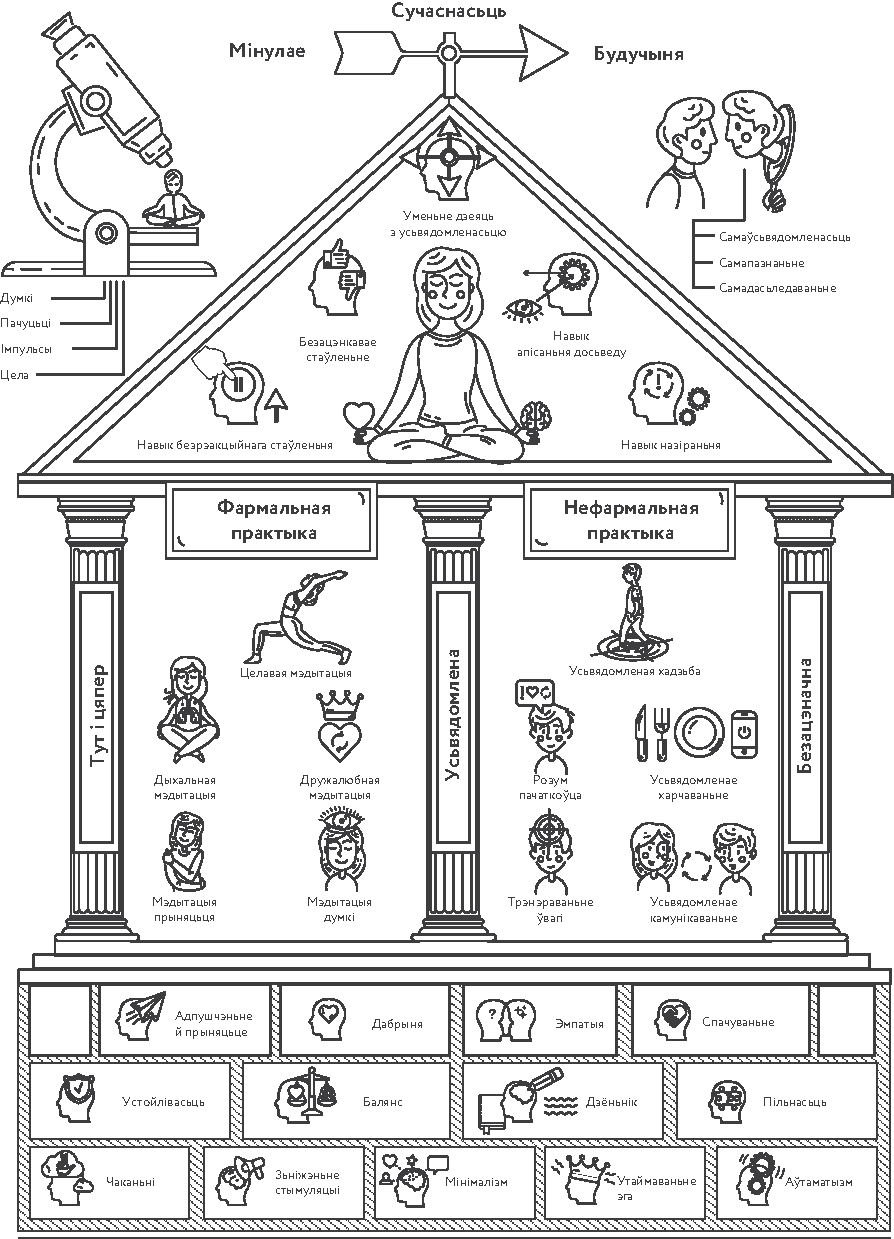
\includegraphics[width=0.95\textwidth]{willpower/ch8/full.pdf}  
\end{figure}
